\documentclass{article}

\usepackage{graphicx} % Required for inserting images
\usepackage{placeins}                             % \FloatBarrier
\usepackage{parskip}                              % no indent
\usepackage{setspace}                             % line spacing, we'll use \setstretch{1.2}
\usepackage[a4paper, bottom=3cm]{geometry}

% TEXT

\usepackage[T1]{fontenc}                        % letters such as ç, ò, etc

\usepackage[backend=biber, style=authoryear]{biblatex}
\addbibresource{refs.bib}

\usepackage{mathtools,amsmath,amssymb,amsthm}   % math symbols, and theorems
\usepackage{dsfont}                             % indicator function
\usepackage{siunitx}                            % writing units (15 h, 10 kg, etc)
\usepackage{xltabular}                          % for xltabular environment
\usepackage{hyperref}
    \hypersetup{
        colorlinks=true,
        linkcolor=blue,
        citecolor=blue,
    }


% TEXT FORMATTING
\usepackage[dvipsnames]{xcolor}                   % colors for the hyperlinks and the parameter table
\usepackage{enumitem}

\newcommand {\Z}{\mathbb{Z}}                    % shortcuts for symbols
\newcommand {\R}{\mathbb{R}}
\newcommand {\diff}{\mathrm{d}}

% parameter table: a value that changed, and an entry that is no longer used
\newcommand {\chg}[1]{\textcolor{BrickRed}{#1}}
\newcommand {\unused}{\textcolor{gray}{\cdot}}

\newtheorem{theorem}{Theorem}                   % theorem environments
\newtheorem{definition}{Definition}
\newtheorem{proposition}{Proposition}
\newtheorem*{proposition*}{Proposition}
\newtheorem{lemma}{Lemma}
\newtheorem{remark}{Remark}
\newtheorem{corollary}{Corollary}
\newtheorem{example}{Example}
\newtheorem{codedef}{Code}
\newtheorem{program}{Program}
\newtheorem{notation}{Notation}


%%%%%%%%%%%%%%%%%%%%%%%%%%%%%%%%%%%%
%       BEGIN DOCUMENT             %
%%%%%%%%%%%%%%%%%%%%%%%%%%%%%%%%%%%%

\begin{document}





%%%%%%%%%%%%%%%%%%%%%%%%%%%%%%%%%%%%
%               TITLE              %
%%%%%%%%%%%%%%%%%%%%%%%%%%%%%%%%%%%%

\newgeometry{top=1.5cm, bottom=1.5cm, left=1.5cm, right=1.5cm}

\title{3D modelling of confined gastruloid aggregates}

% \author{
%     David Oriola$^{1}$,
%     Víctor Villegas-Morral$^{1}$,
%     Vanessa Weichselberger$^{2}$,
%     \\[1.5ex]
%     \small $^{1}$Universitat Politècnica de Catalunya,\
%     \small $^{3}$EMBL
% }

\date{\today}

% manual title: \maketitle leaves an empty author line when \author is unset
\begin{center}
    {\LARGE 3D modelling of confined gastruloid aggregates\par}
    \vspace{0.5em}
    {\large \today\par}
\end{center}




%%%%%%%%%%%%%%%%%%%%%%%%%%%%%%%%%%%%
%       OVERVIEW                   %
%%%%%%%%%%%%%%%%%%%%%%%%%%%%%%%%%%%%

\begin{figure}[!h]
    \centering
    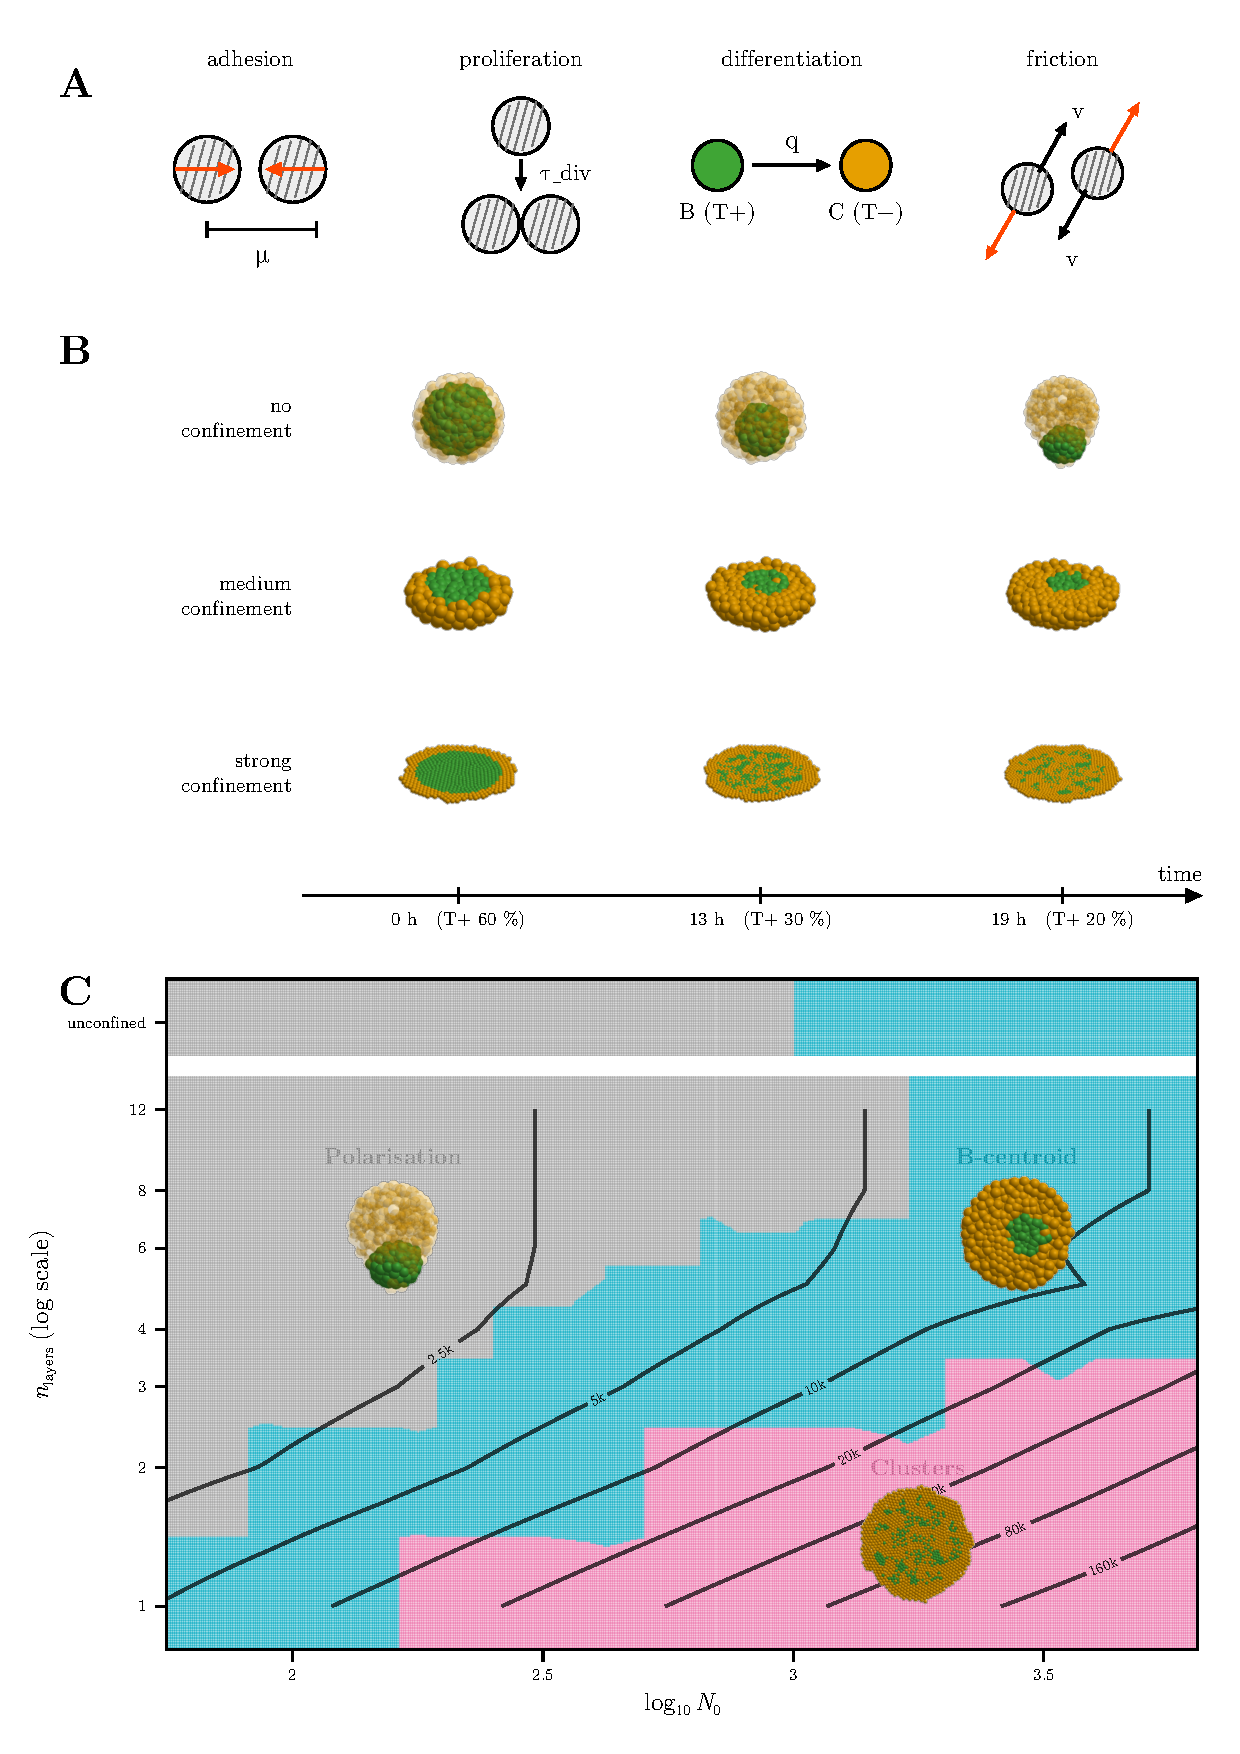
\includegraphics[width=0.82\linewidth]{figures/overview.pdf}
    \caption{Overview. 
        (A) Model ingredients. 
        (B) Evolution of same aggregate ($N_0=600$ cells) without confinement, with medium confinement (4 layers) and with strong confinement (1 layer).
        (C) Outcome phase space: number of initial cells against the number of layers between the plates, read when $20\%$ of the cells are $B$. Lines: area of the pancake at squeezing ($\mu$m$^2$). Each example sits on its region: the last frames of the rows of (B).}
    \label{fig:overview}
\end{figure}




%%%%%%%%%%%%%%%%%%%%%%%%%%%%%%%%%%%%
%     TABLE OF CONTENTS            %
%%%%%%%%%%%%%%%%%%%%%%%%%%%%%%%%%%%%

\clearpage
\restoregeometry
\setcounter{tocdepth}{1}
\tableofcontents




%%%%%%%%%%%%%%%%%%%%%%%%%%%%%%%%%%%%
%           TEXT                   %
%%%%%%%%%%%%%%%%%%%%%%%%%%%%%%%%%%%%

\section{The experiment}

In the expriments, they grow a gastruloid and confine it right before polarisation should occur. Cells transition $A\to B\to C$, and in that moment the distribution is something like: almost no $A$-cells, a centroid of $B$-cells, and an outer layer mainly formed of $C$-cells. On squeezing the aggregate between two plates, there are three possible outcomes.
\begin{enumerate}
    \item If the confinement is strong enough (i.e. small plate distance), the centroid starts disintegrating usually forming a ring-like structure and then breaks into clusters.
    \item For medium confinement, the centroid does not polarise nor breaks into clusters and eventually differentiates away. It may form a ring-like pattern but without breaking.
    \item For weak confinement, the centroid polarises as when there is no confinement.
\end{enumerate}
Determining whether confinement is strong or weak is not trivial and is actually key to this research. The experiments observe that the larger the intitial size on squeezing, the most layers we also get clusters with.

\begin{figure}[h]
    \centering
    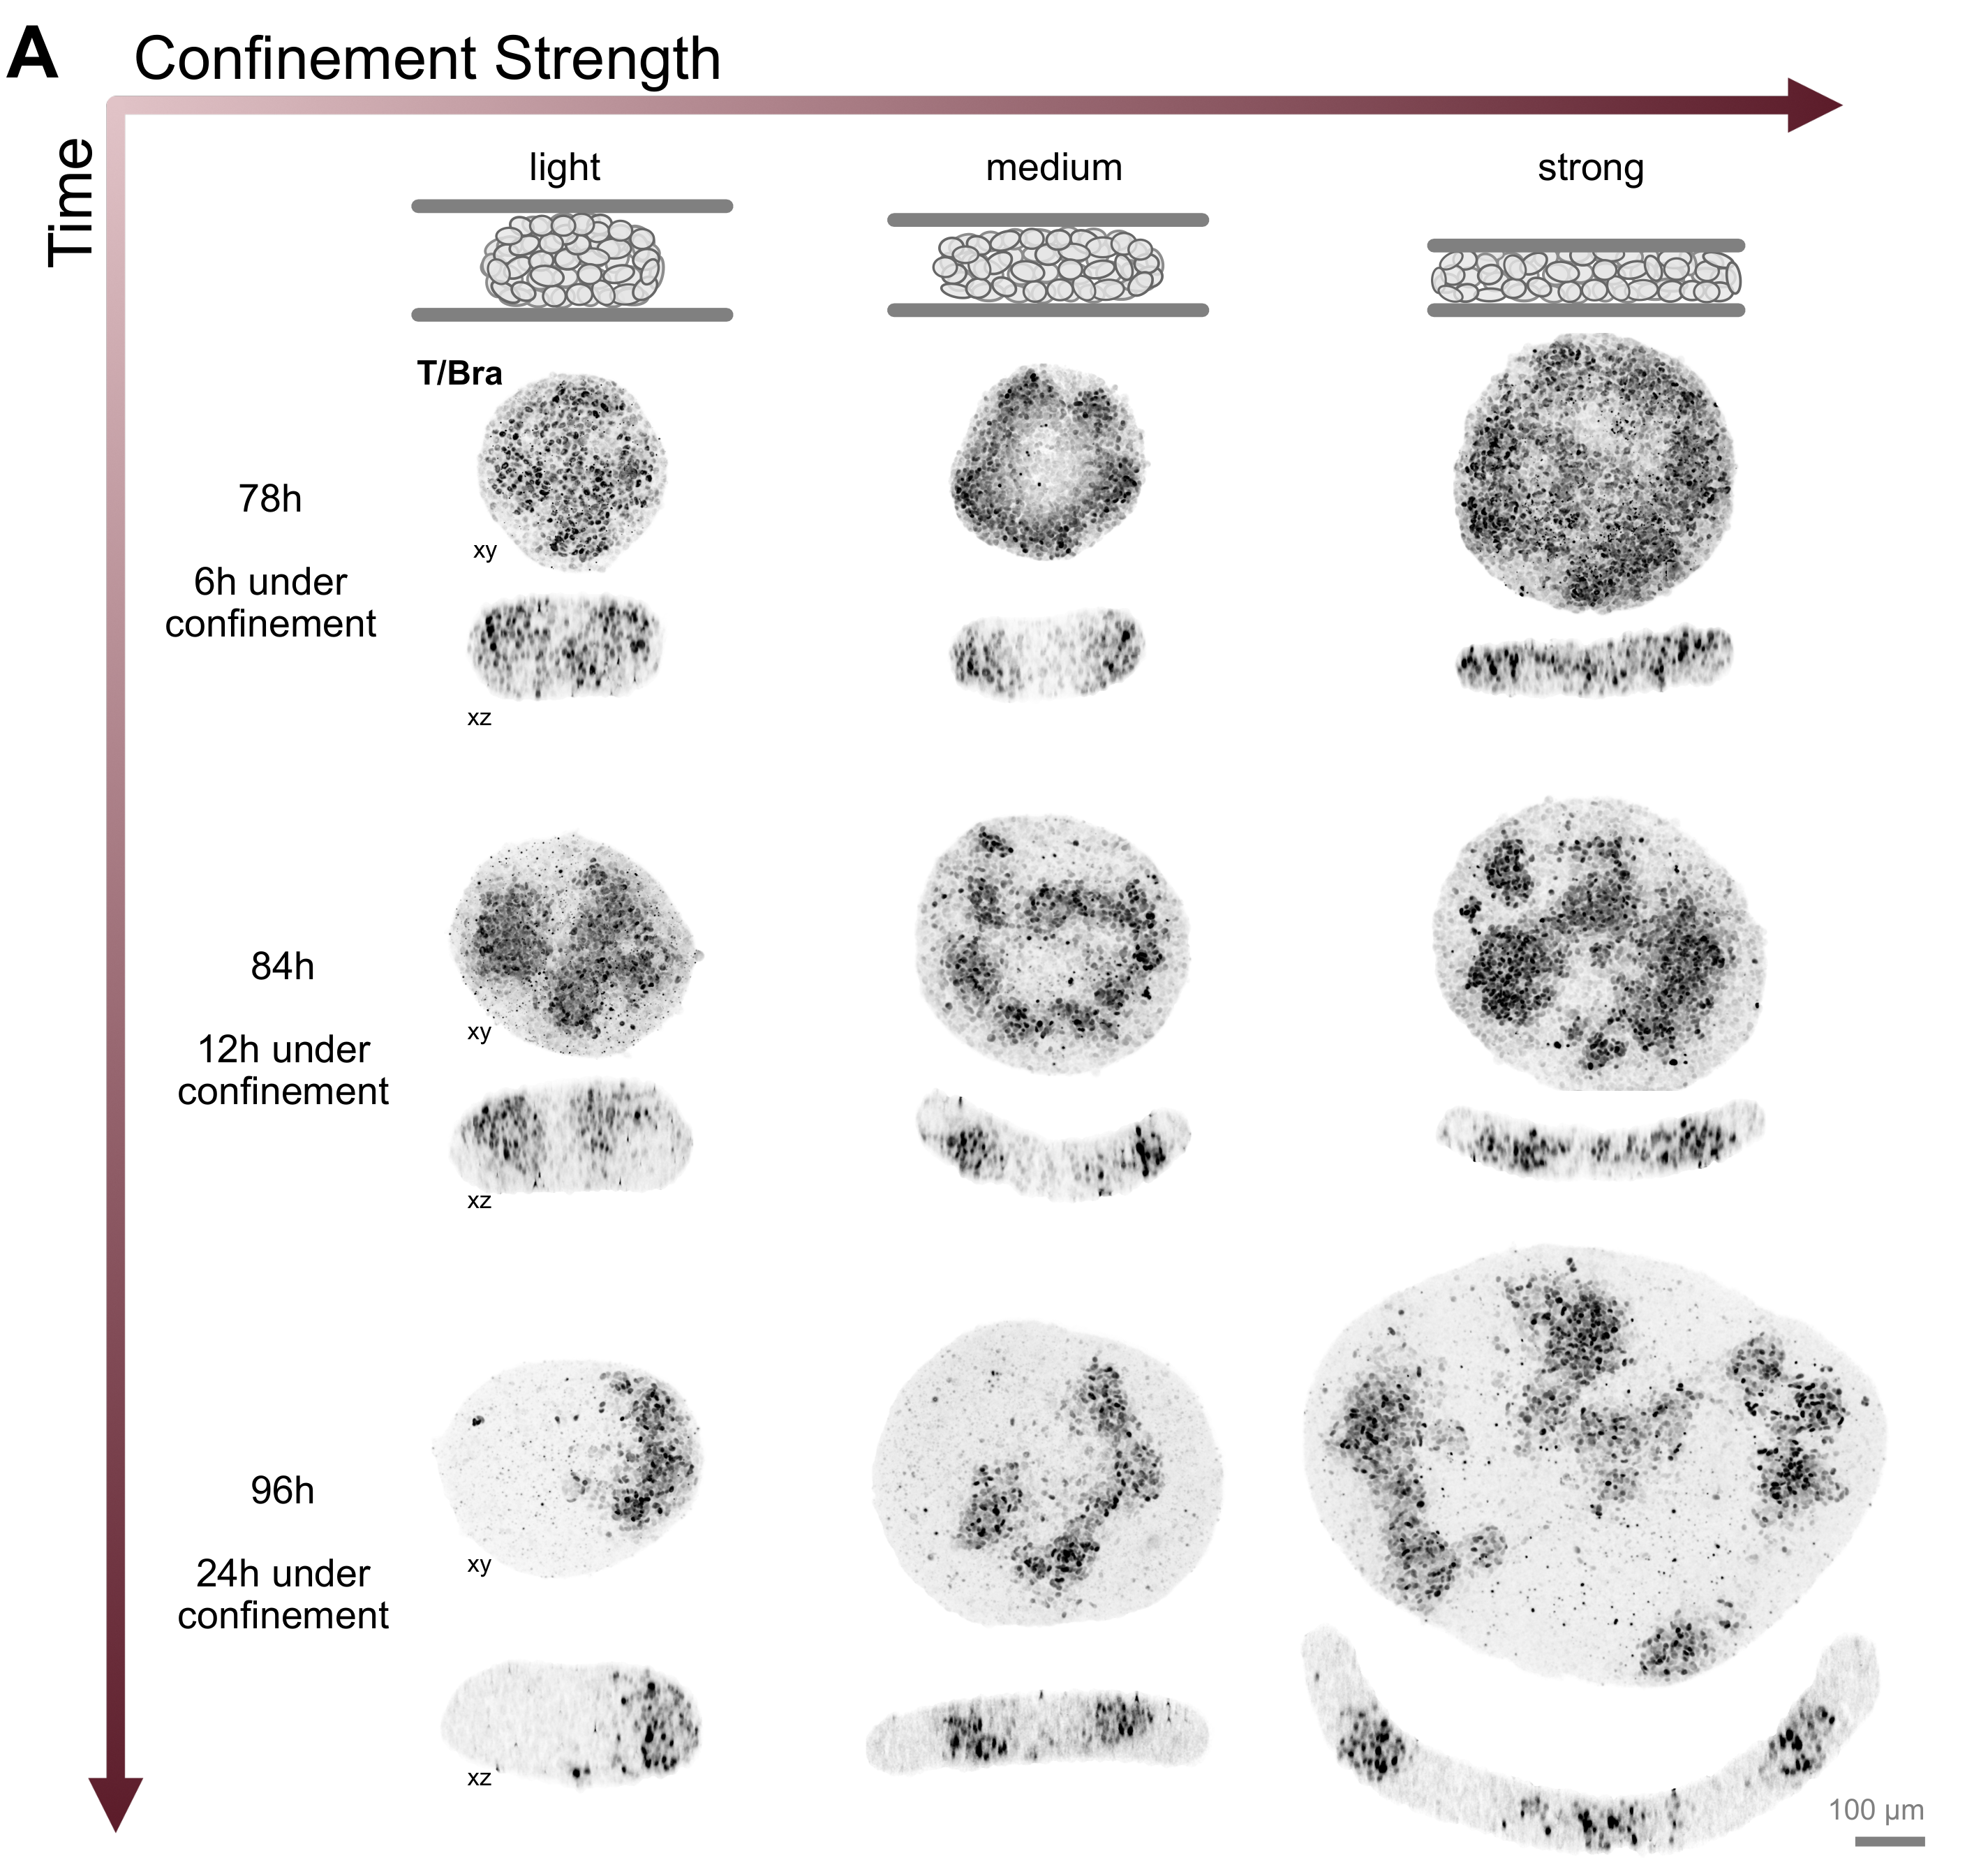
\includegraphics[width=0.65\linewidth]{figures/exp-confinement-time.png}
    \caption{
        T/Bra patterning under light, medium and strong confinement (columns) at 78\,h, 84\,h and 96\,h, i.e.\ 6\,h, 12\,h and 24\,h under confinement (rows).
        Each aggregate is shown from the top (xy) and from the side (xz).
        Light confinement keeps a pole, medium confinement keeps the T/Bra cells in the centre and strong confinement breaks them into clusters.
        From V.~Weichselberger's poster.}
    \label{fig:exp-confinement-time}
\end{figure}

The experimentalists image the aggregate and track the cells in order to perform certain measurements.

\begin{figure}[h]
    \centering
    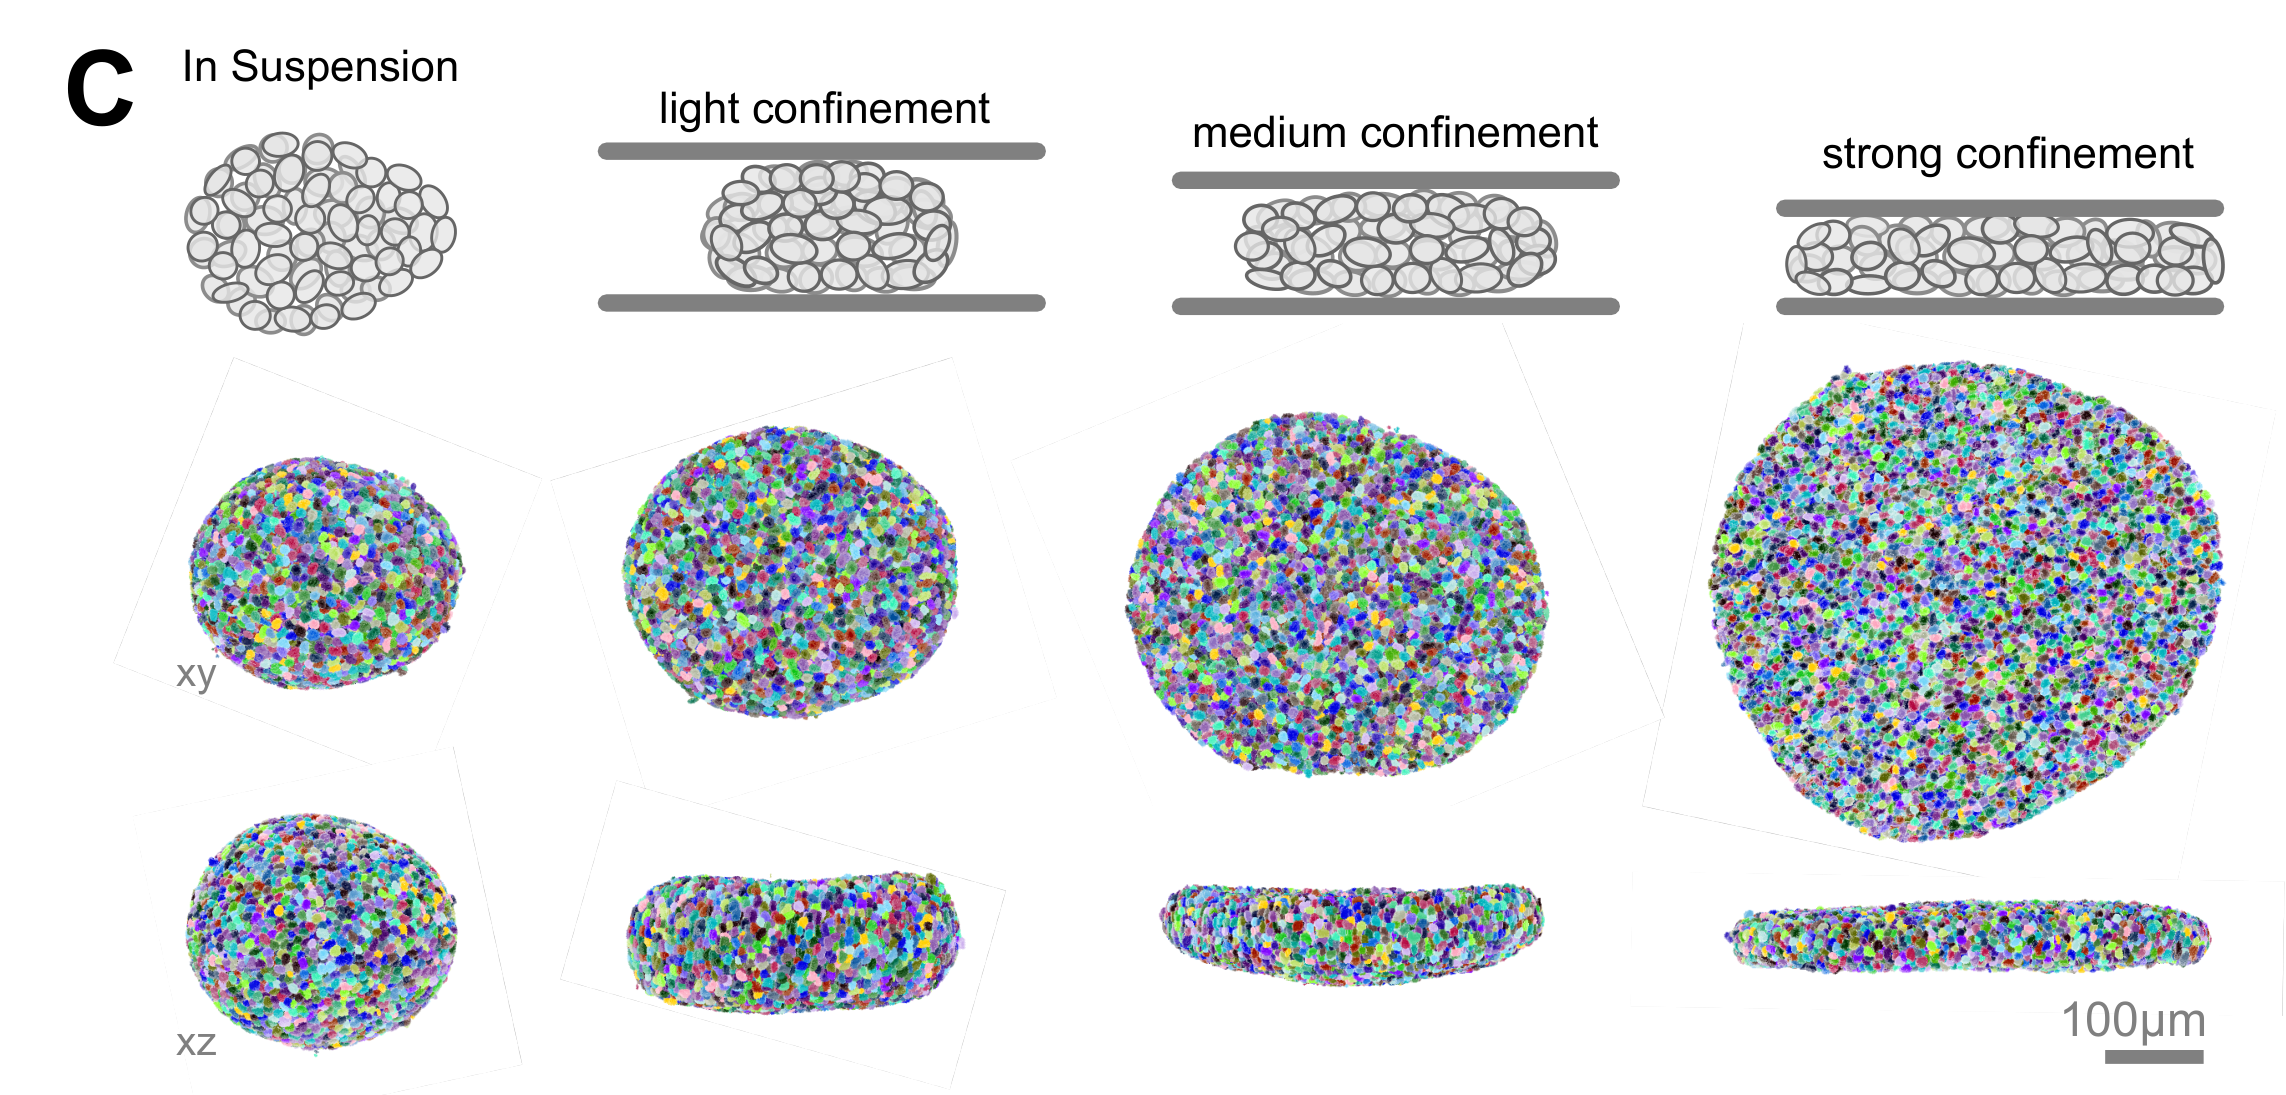
\includegraphics[width=0.7\linewidth]{figures/exp-segmentation.png}
    \caption{
        3D segmentation of gastruloids after 24\,h in suspension or under light, medium and strong confinement, seen from the top (xy) and from the side (xz).
        From V.~Weichselberger's poster.}
    \label{fig:exp-segmentation}
\end{figure}

\begin{figure}[h]
    \centering
    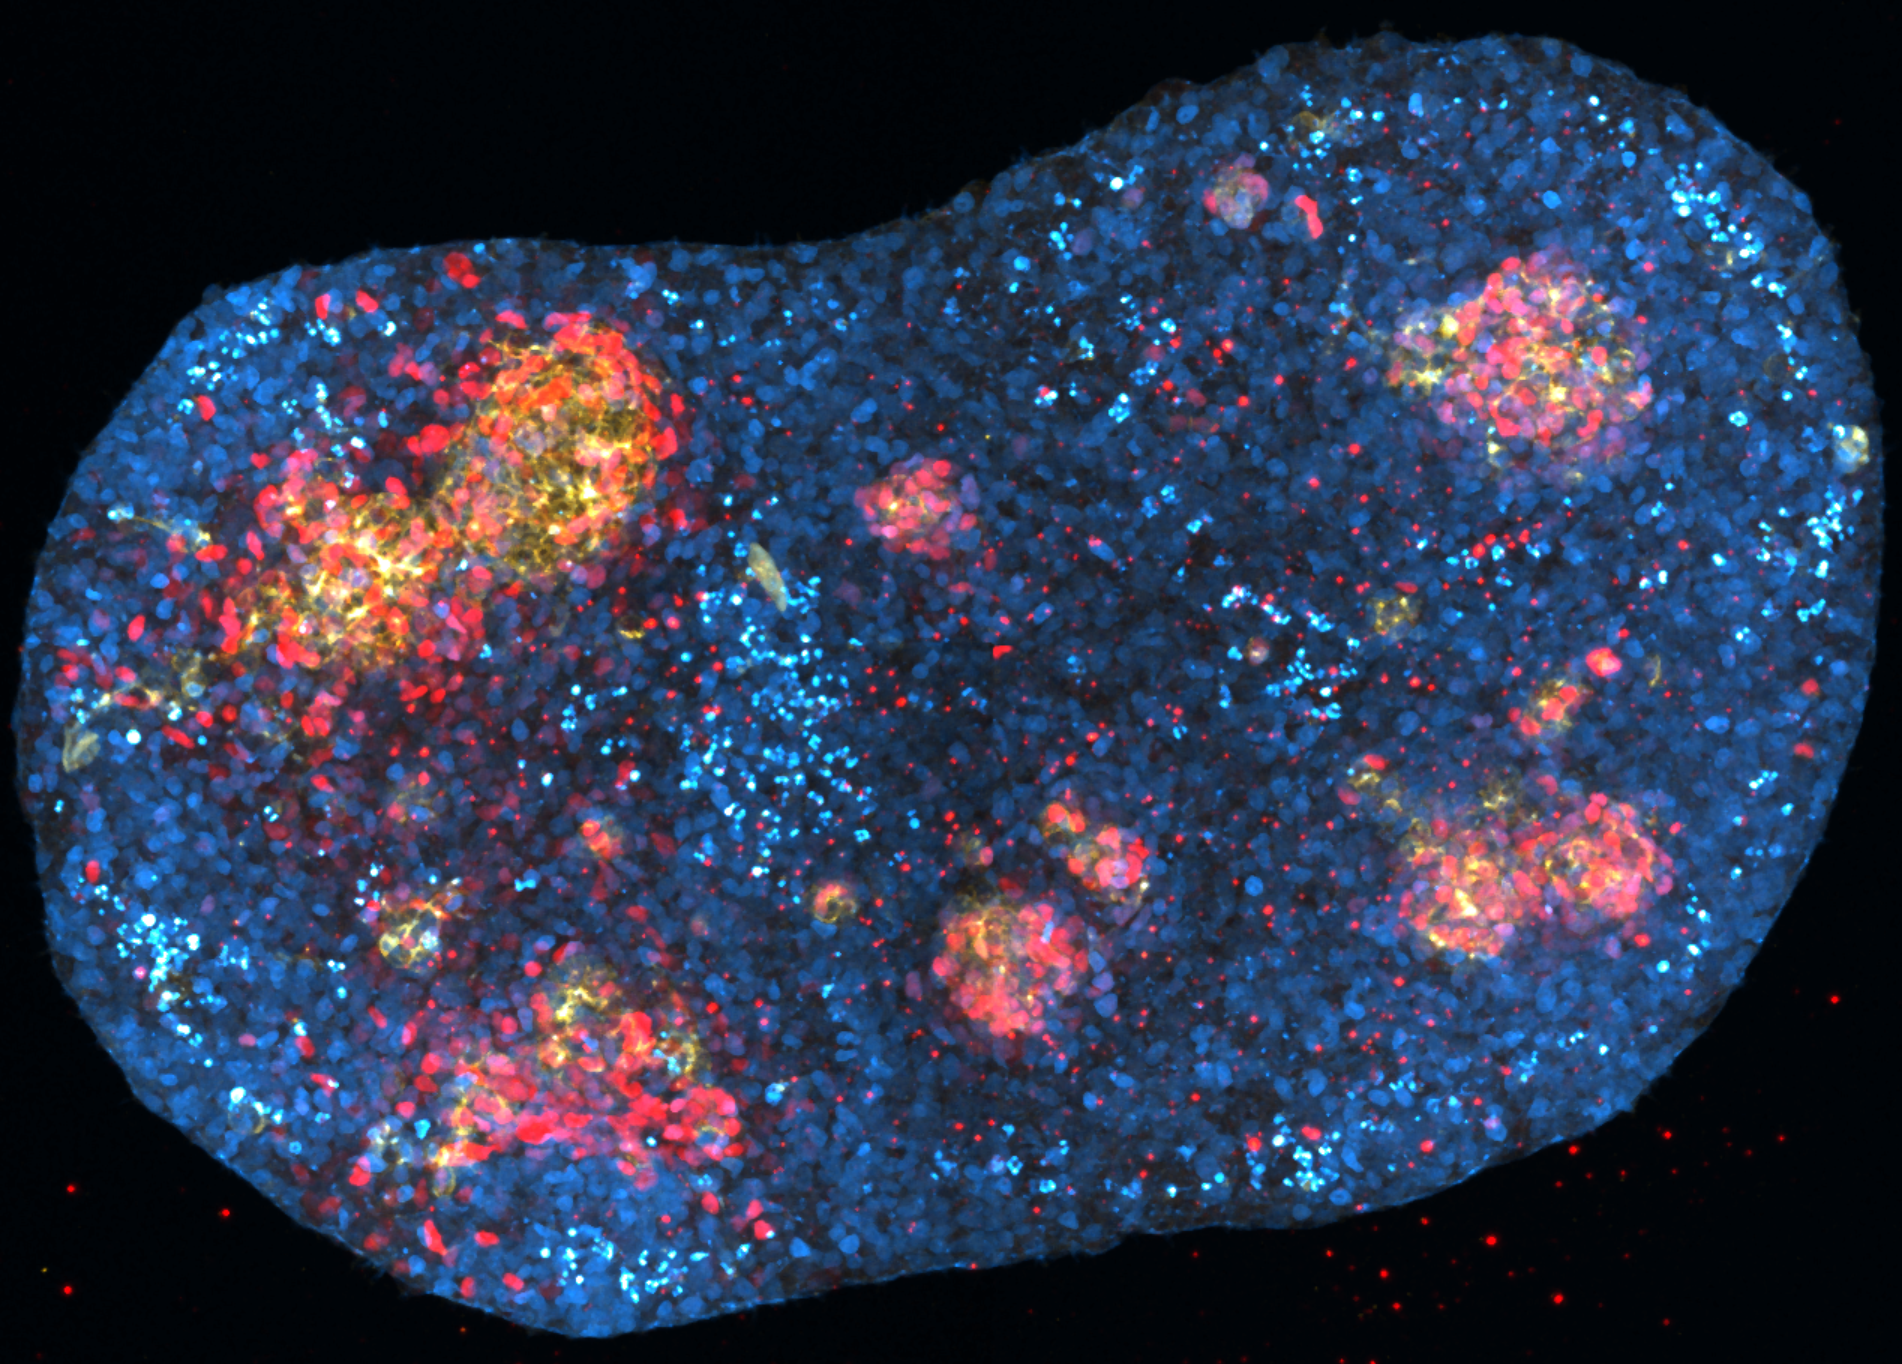
\includegraphics[width=0.32\linewidth]{figures/exp-microscopy.png}

    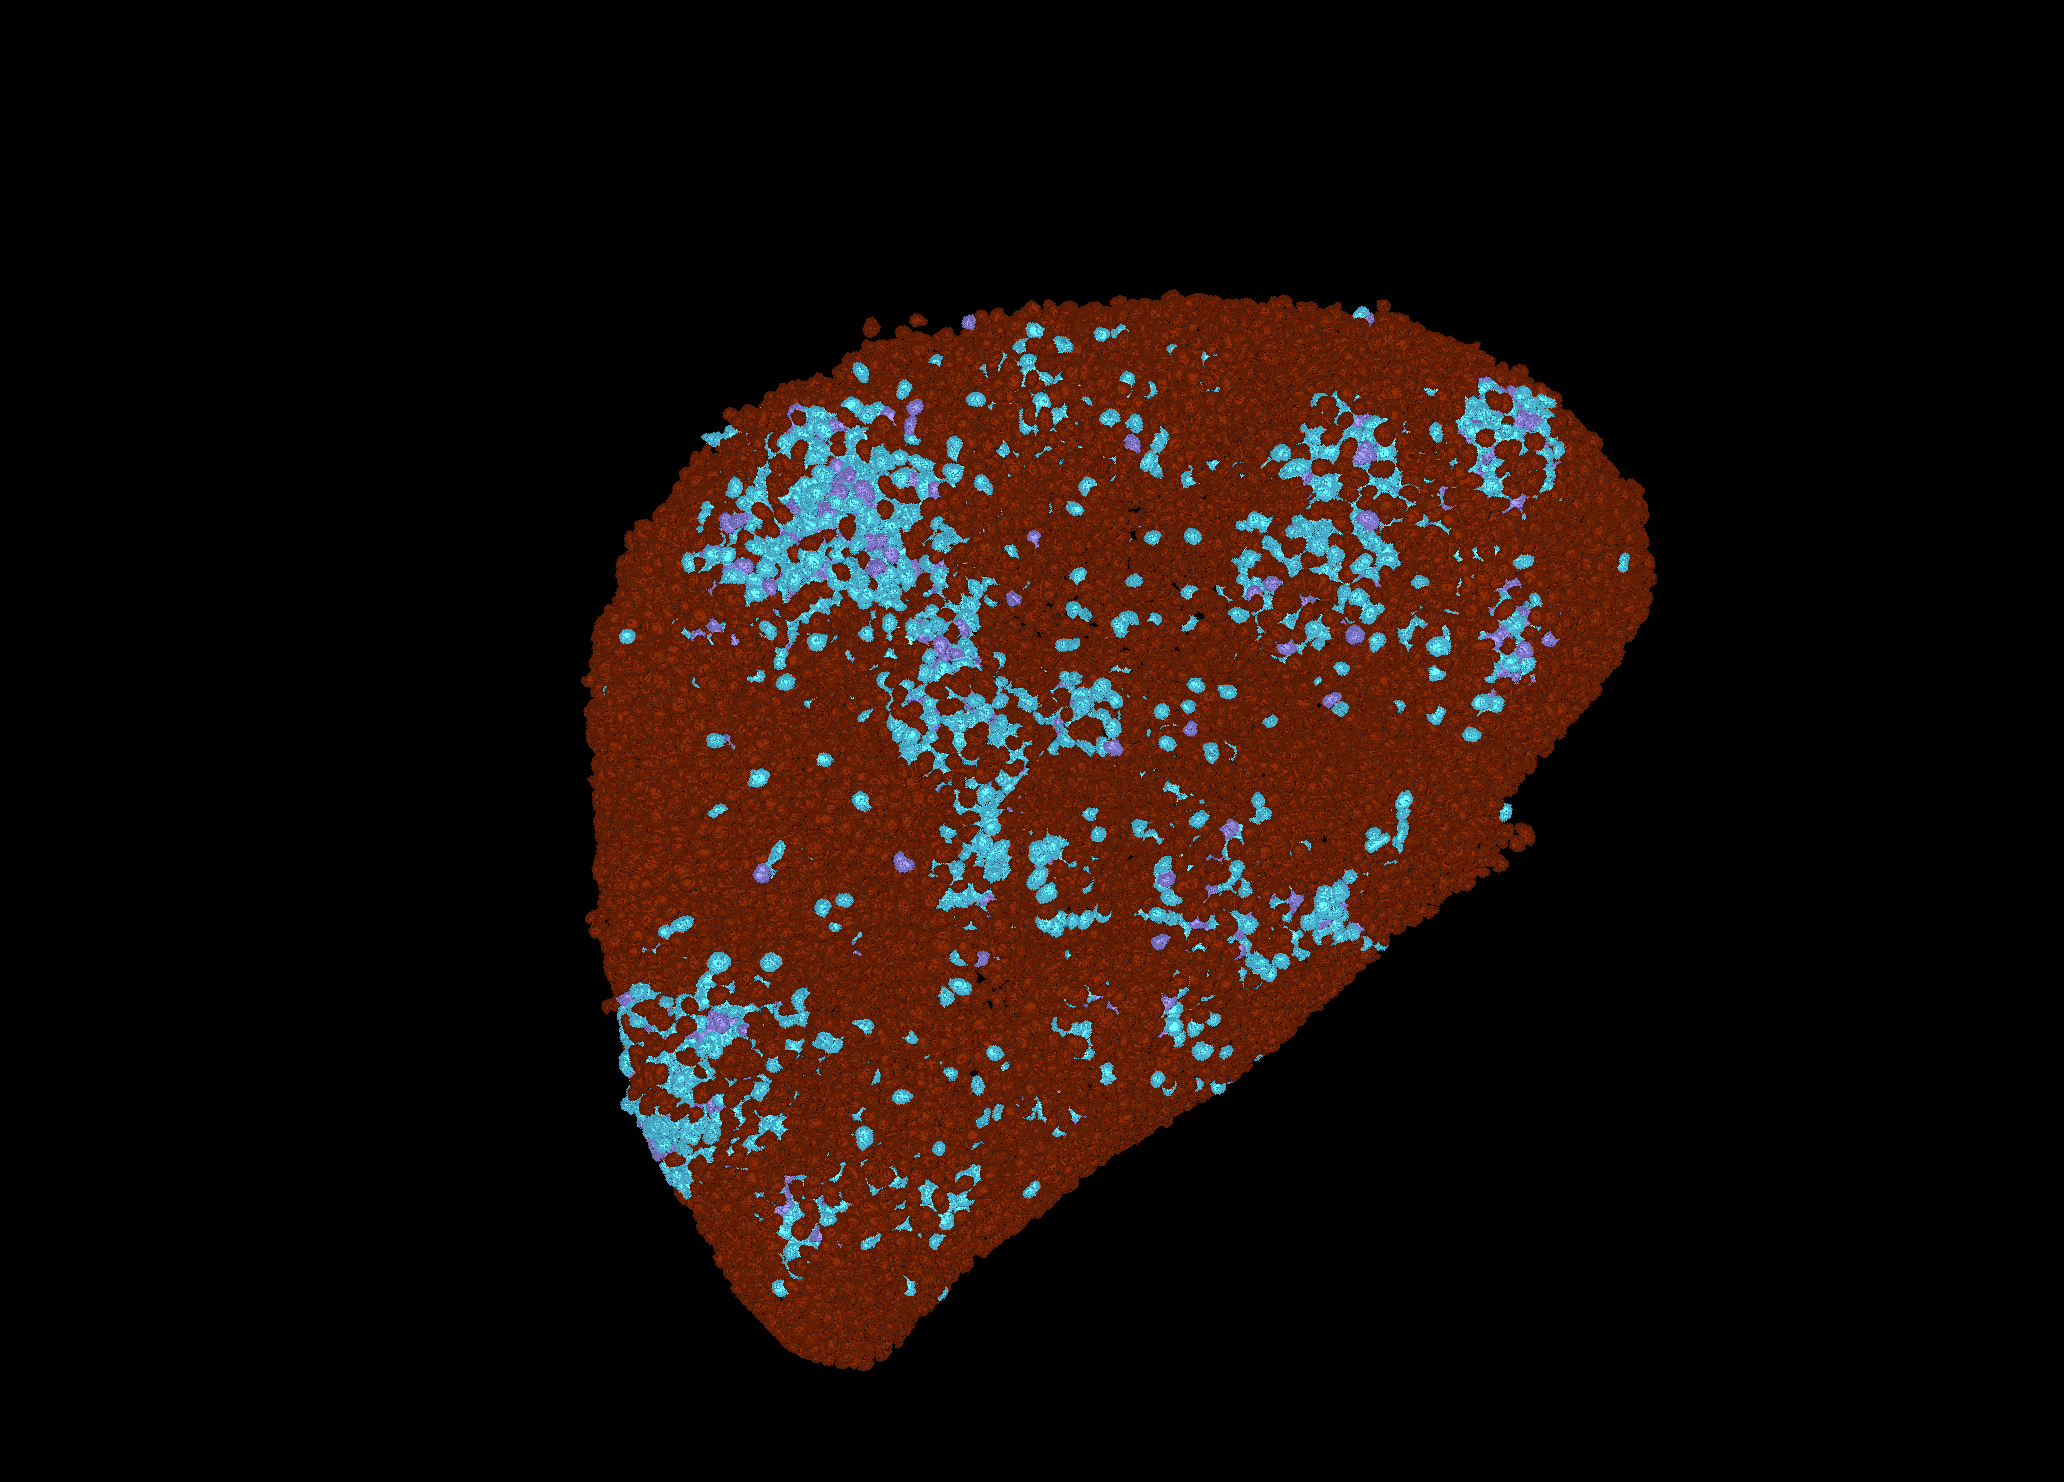
\includegraphics[width=0.32\linewidth]{figures/exp-segmented-1.png}
    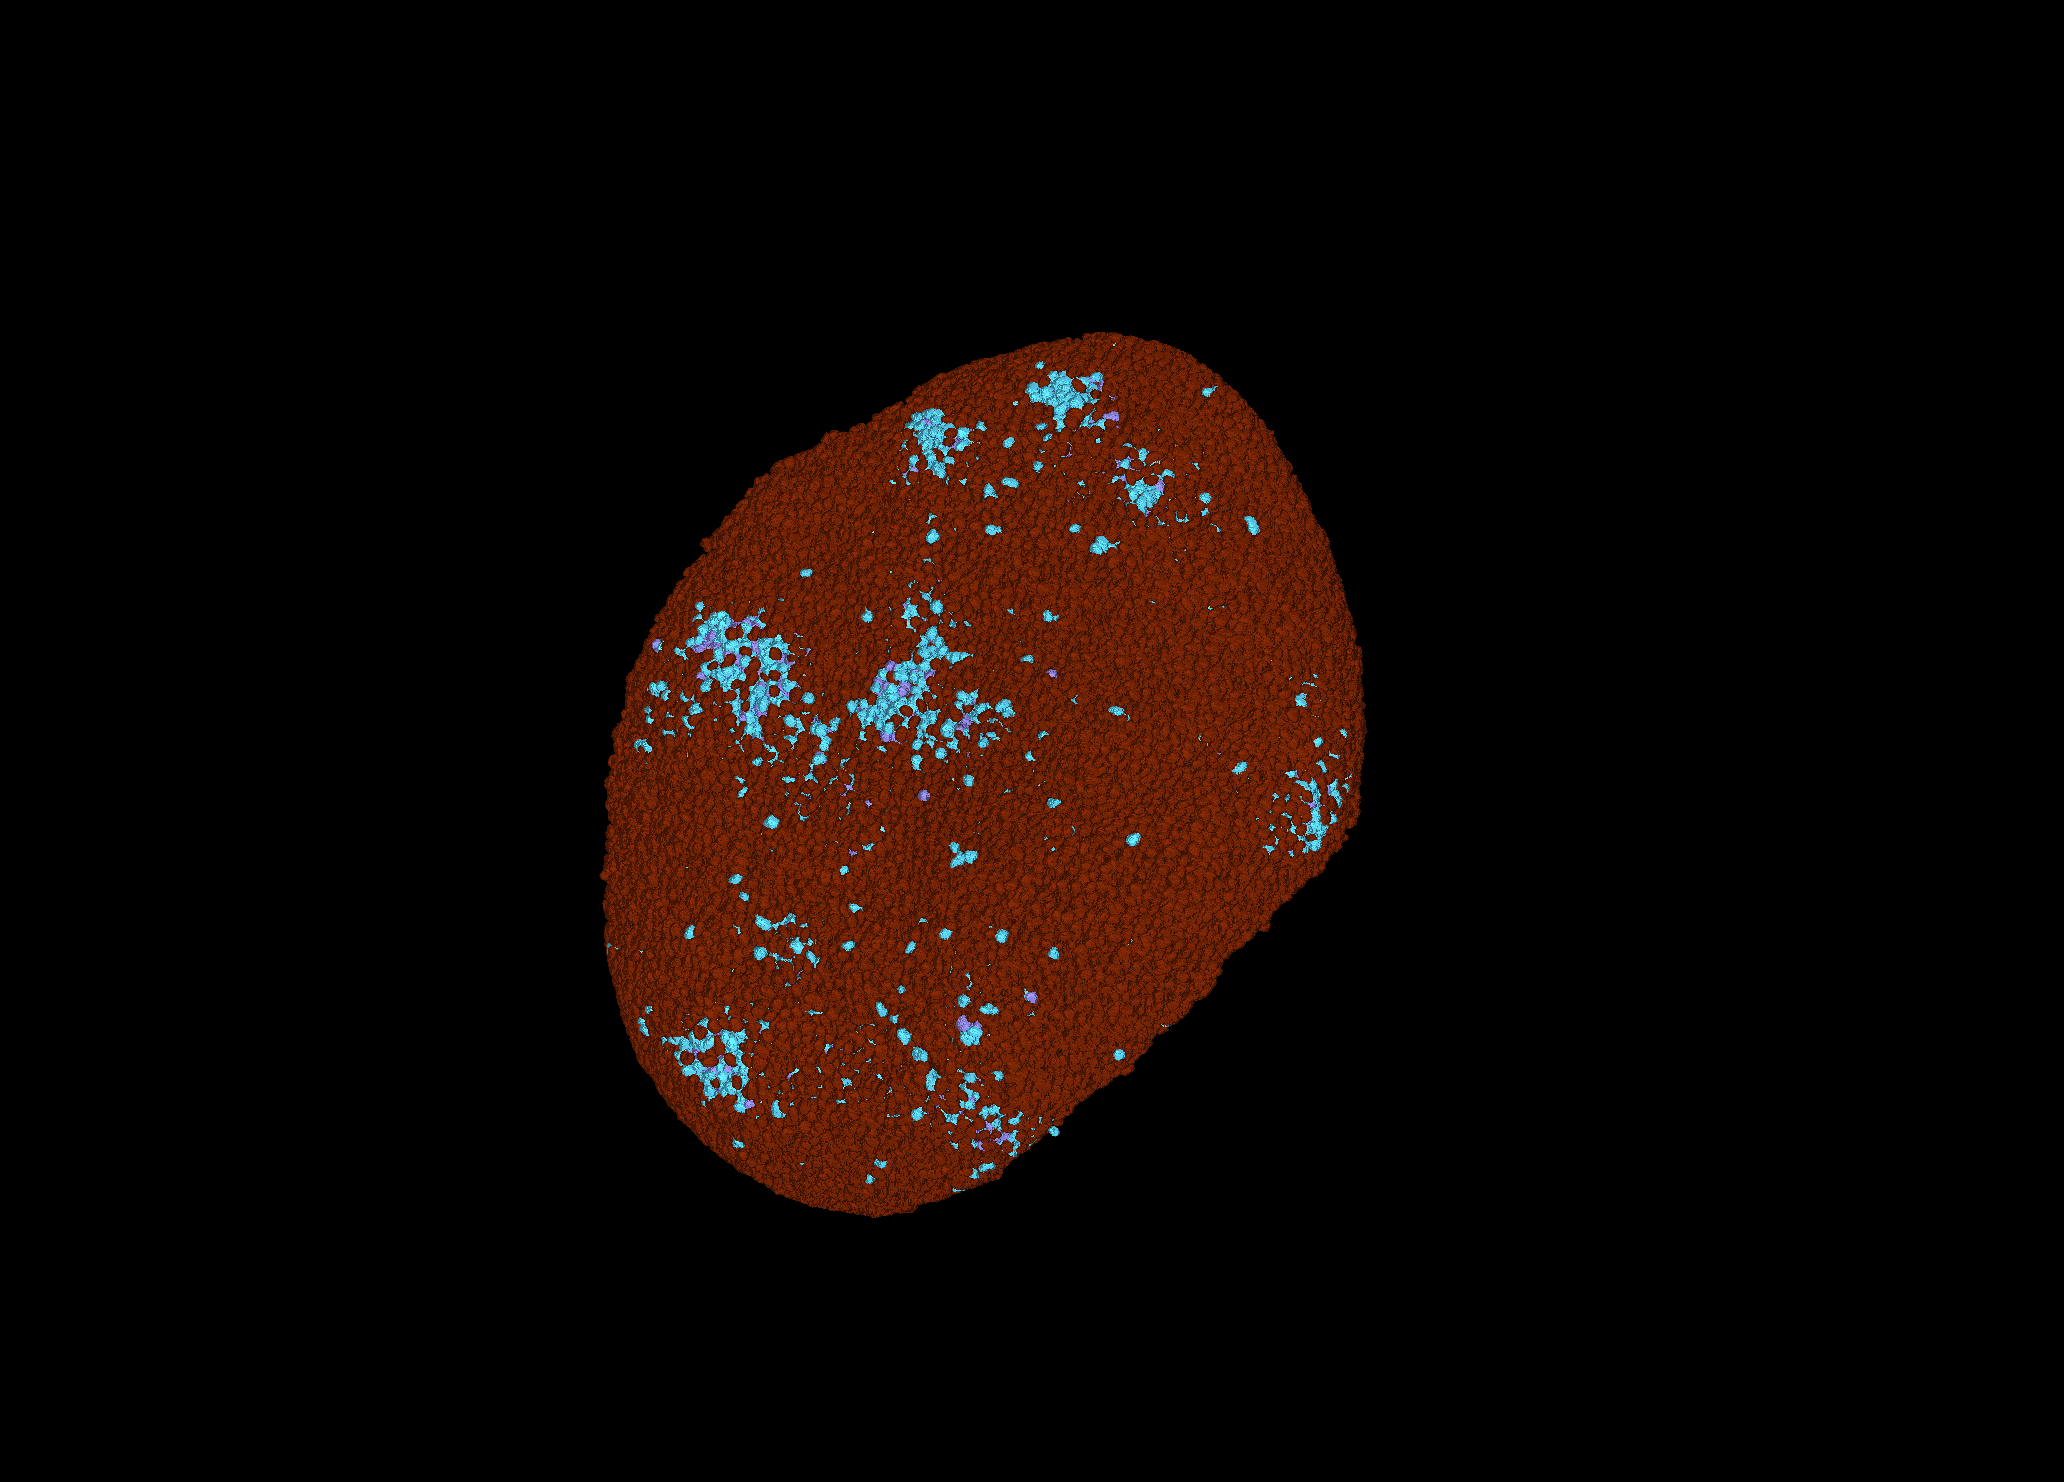
\includegraphics[width=0.32\linewidth]{figures/exp-segmented-2.png}
    \caption{
        Confined gastruloids in the experiments.
        Top: microscopy image of an aggregate with several T/Bra clusters (T/Bra in orange, nuclei in blue).
        Bottom: two segmented aggregates, with T/Bra-positive cells in light blue.}
    \label{fig:exp-aggregates}
\end{figure}


\paragraph{Spatial cluster quantification.} It is used to determine whether clusters have formed.

Spatial clustering was quantified using a density-based clustering approach adapted from DBSCAN (Density-Based Spatial Clustering of Applications with Noise). Clusters were identified based on the local enrichment and spatial connectivity of cells belonging to the cell type B population. For each cell, the fraction of neighbouring cells belonging to the same population was calculated within a defined three-dimensional Euclidean radius of 13 µm, considering all surrounding cells as the reference. Cells for which at least $40\%$ of neighbouring cells belonged to the population of interest were defined as core cells. Core cells were grouped into the same cluster if they were directly or indirectly connected through other core cells within a maximum pairwise distance of 13 µm. Cells belonging to the population of interest that did not fulfil the core-cell criterion were assigned as border cells to the cluster of their nearest core cell, provided that this core cell was located within 13 µm. Only clusters containing at least 20 cells, including core and border cells, were retained for further analysis. Clustering was quantified based on the number of clusters, the fraction of cells assigned to clusters, cluster sizes, and the effective number of clusters ($N_\text{eff}$), which accounts for differences in cluster size distribution. The latter was calculated as $N_\text{eff} = \frac{1}{\sum p_i ^2}$, where $p_i$ represents the fraction of all clustered cells belonging to cluster i, providing a measure of cluster number that accounts for differences in cluster size.

\begin{figure}[h]
    \centering
    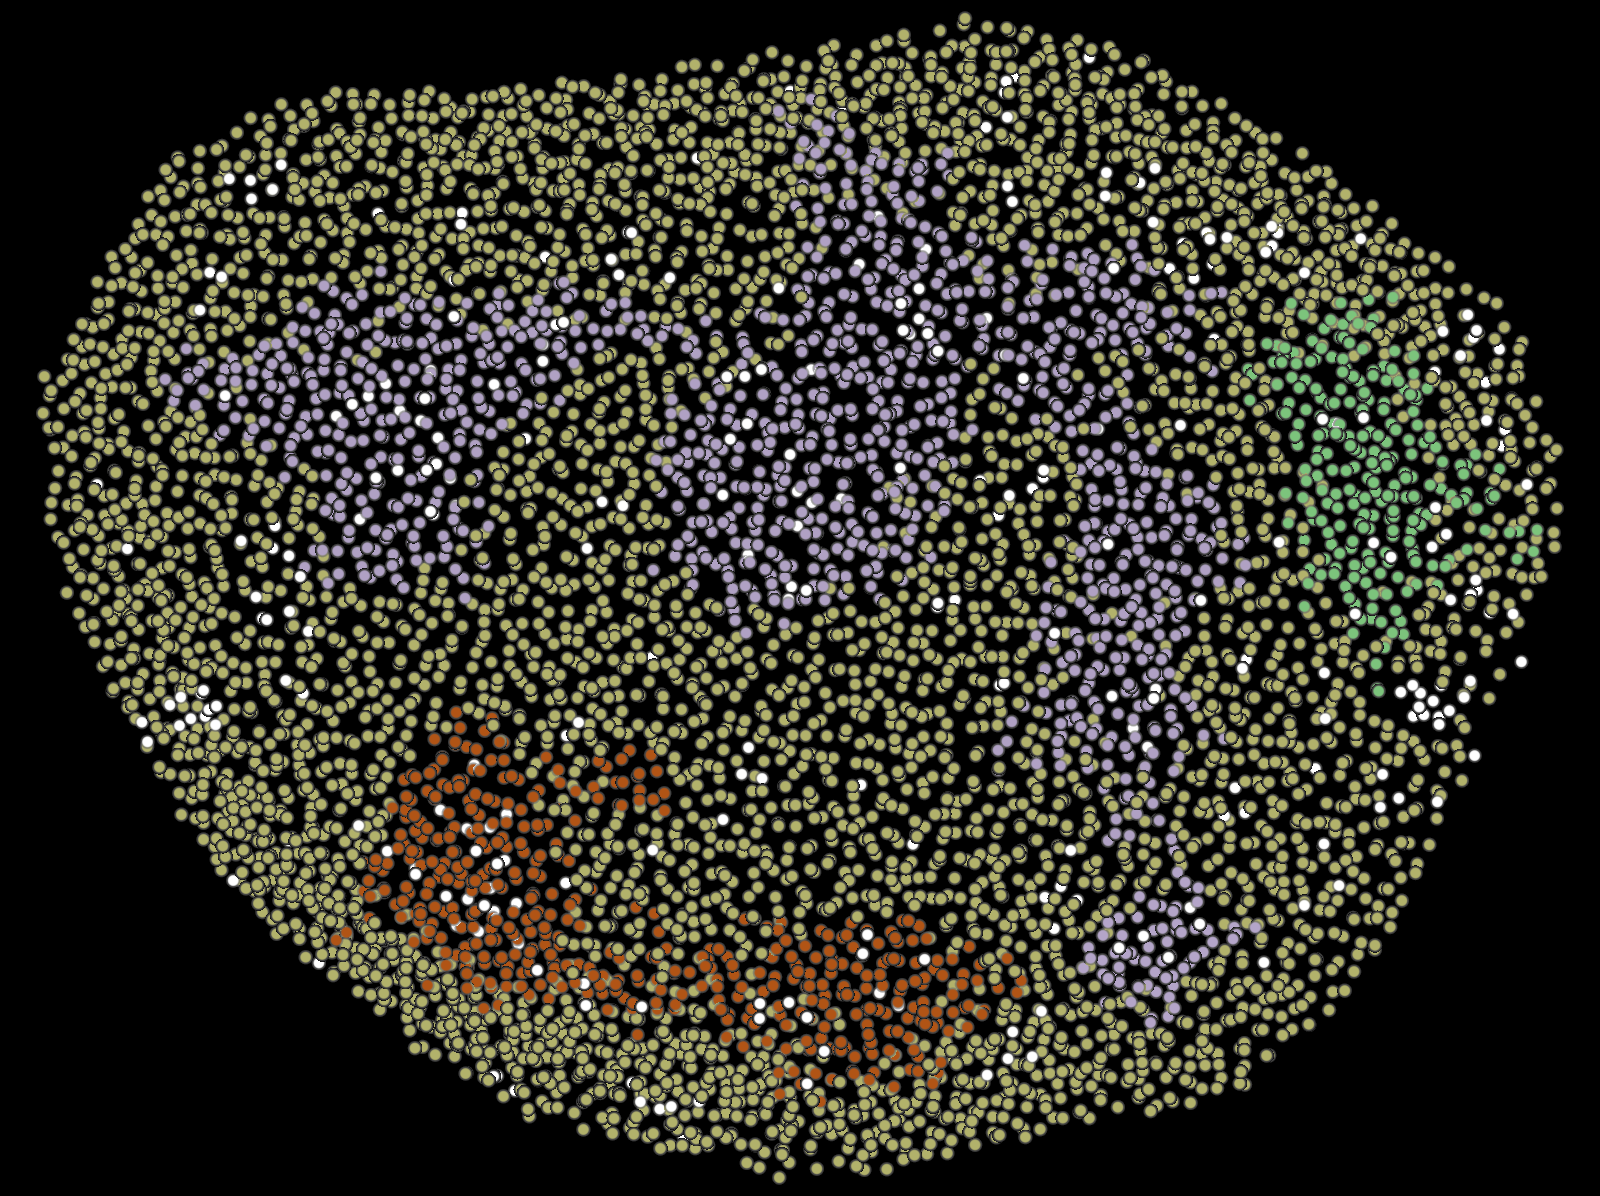
\includegraphics[width=0.32\linewidth]{figures/exp-clusters-1-all.png}
    \hfill
    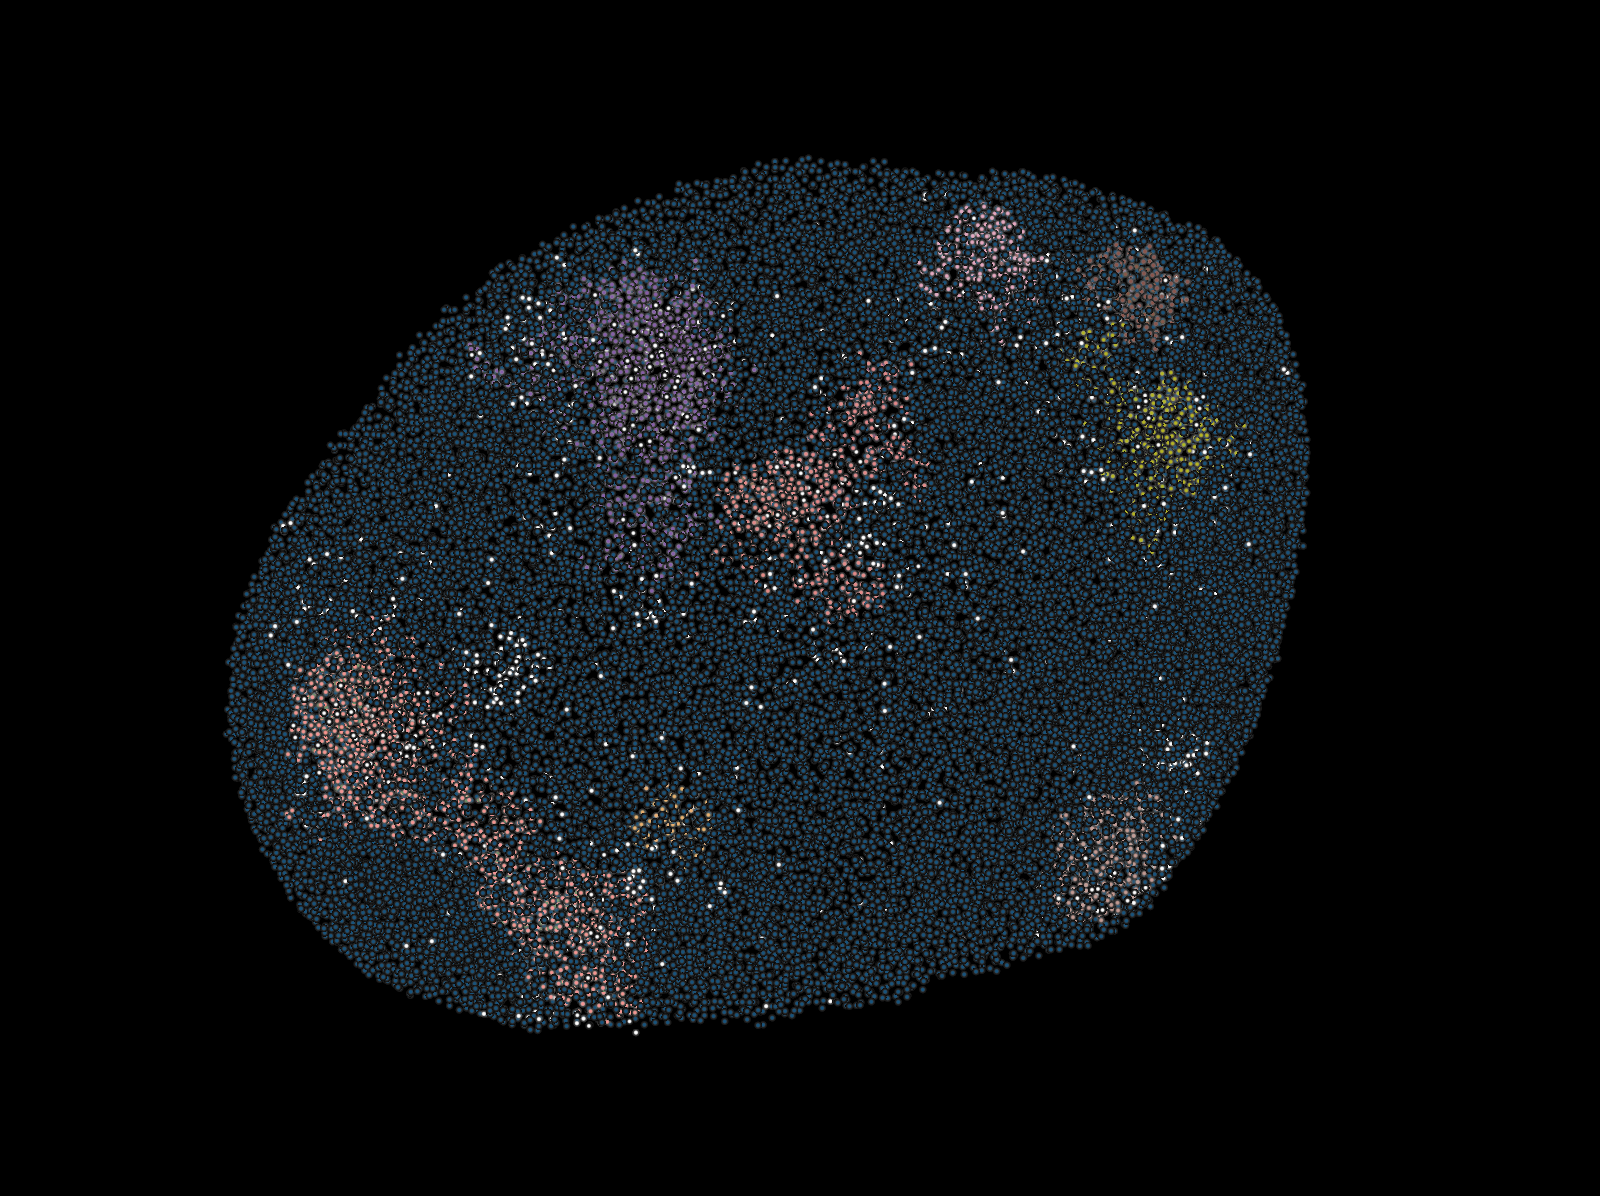
\includegraphics[width=0.32\linewidth]{figures/exp-clusters-2-all.png}
    \hfill
    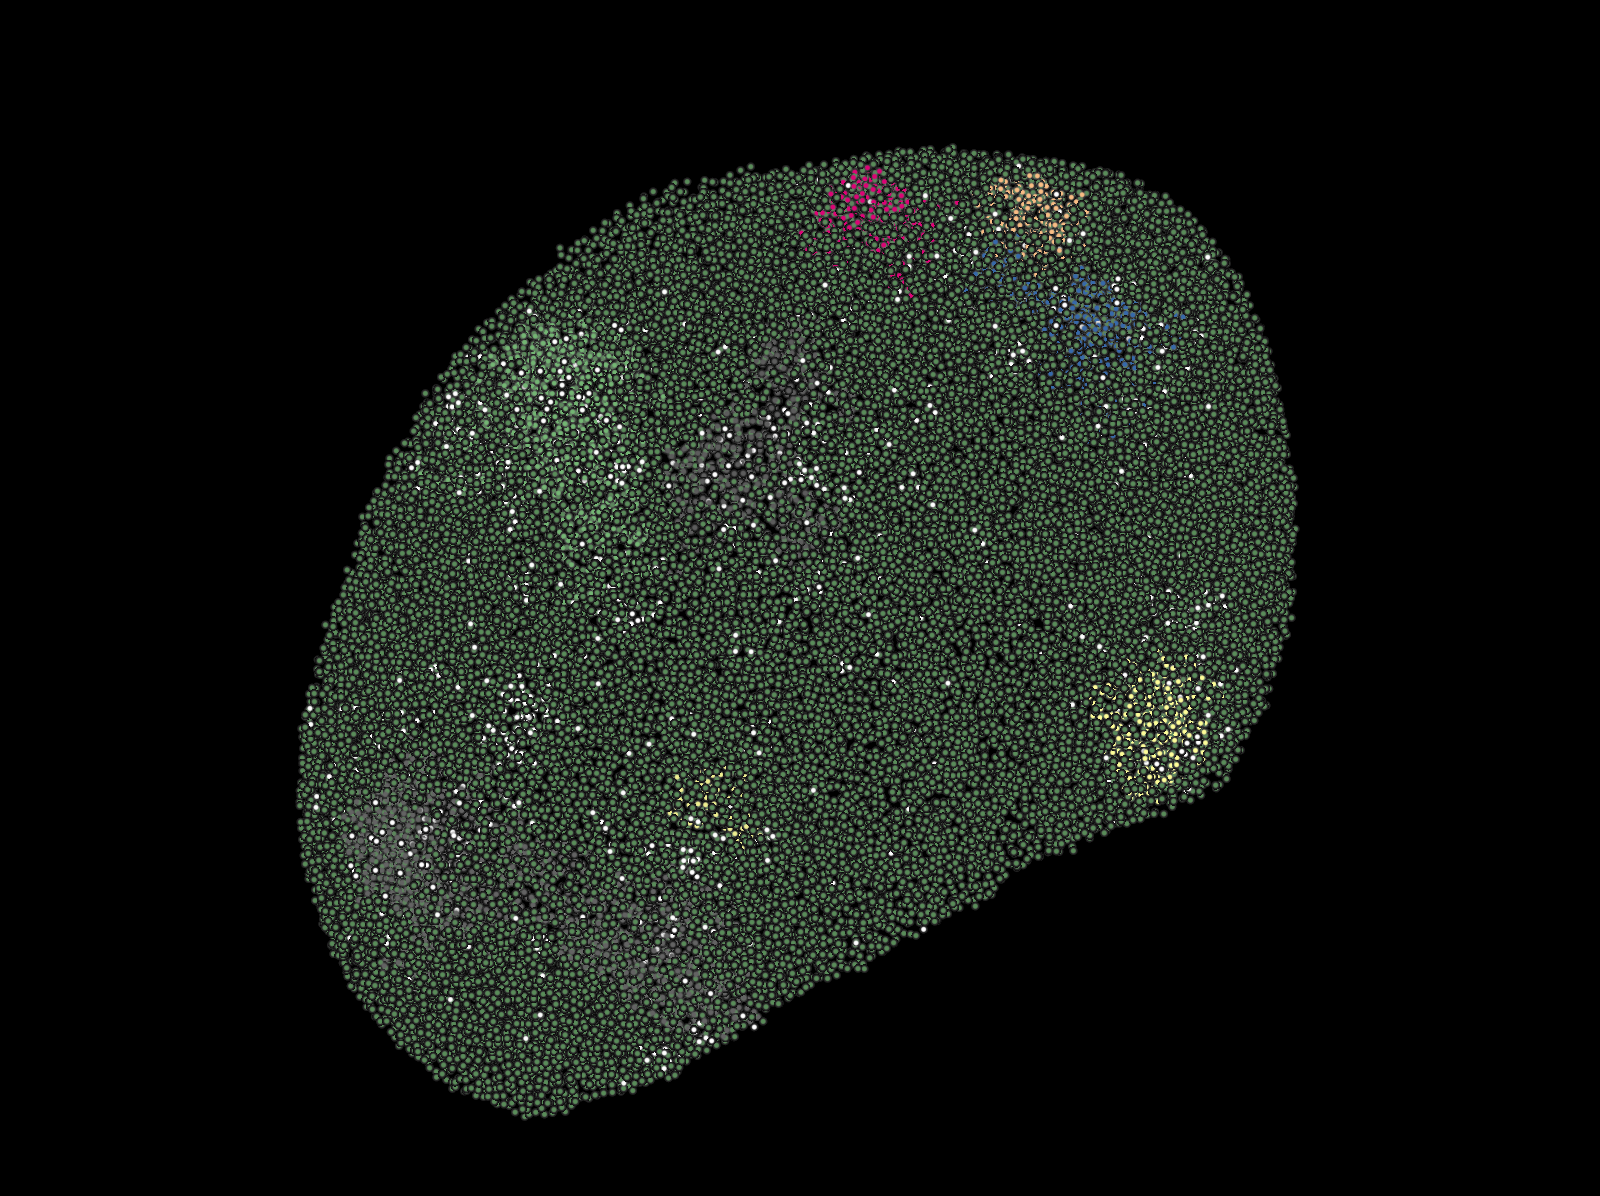
\includegraphics[width=0.32\linewidth]{figures/exp-clusters-3-all.png}

    \vspace{0.5em}
    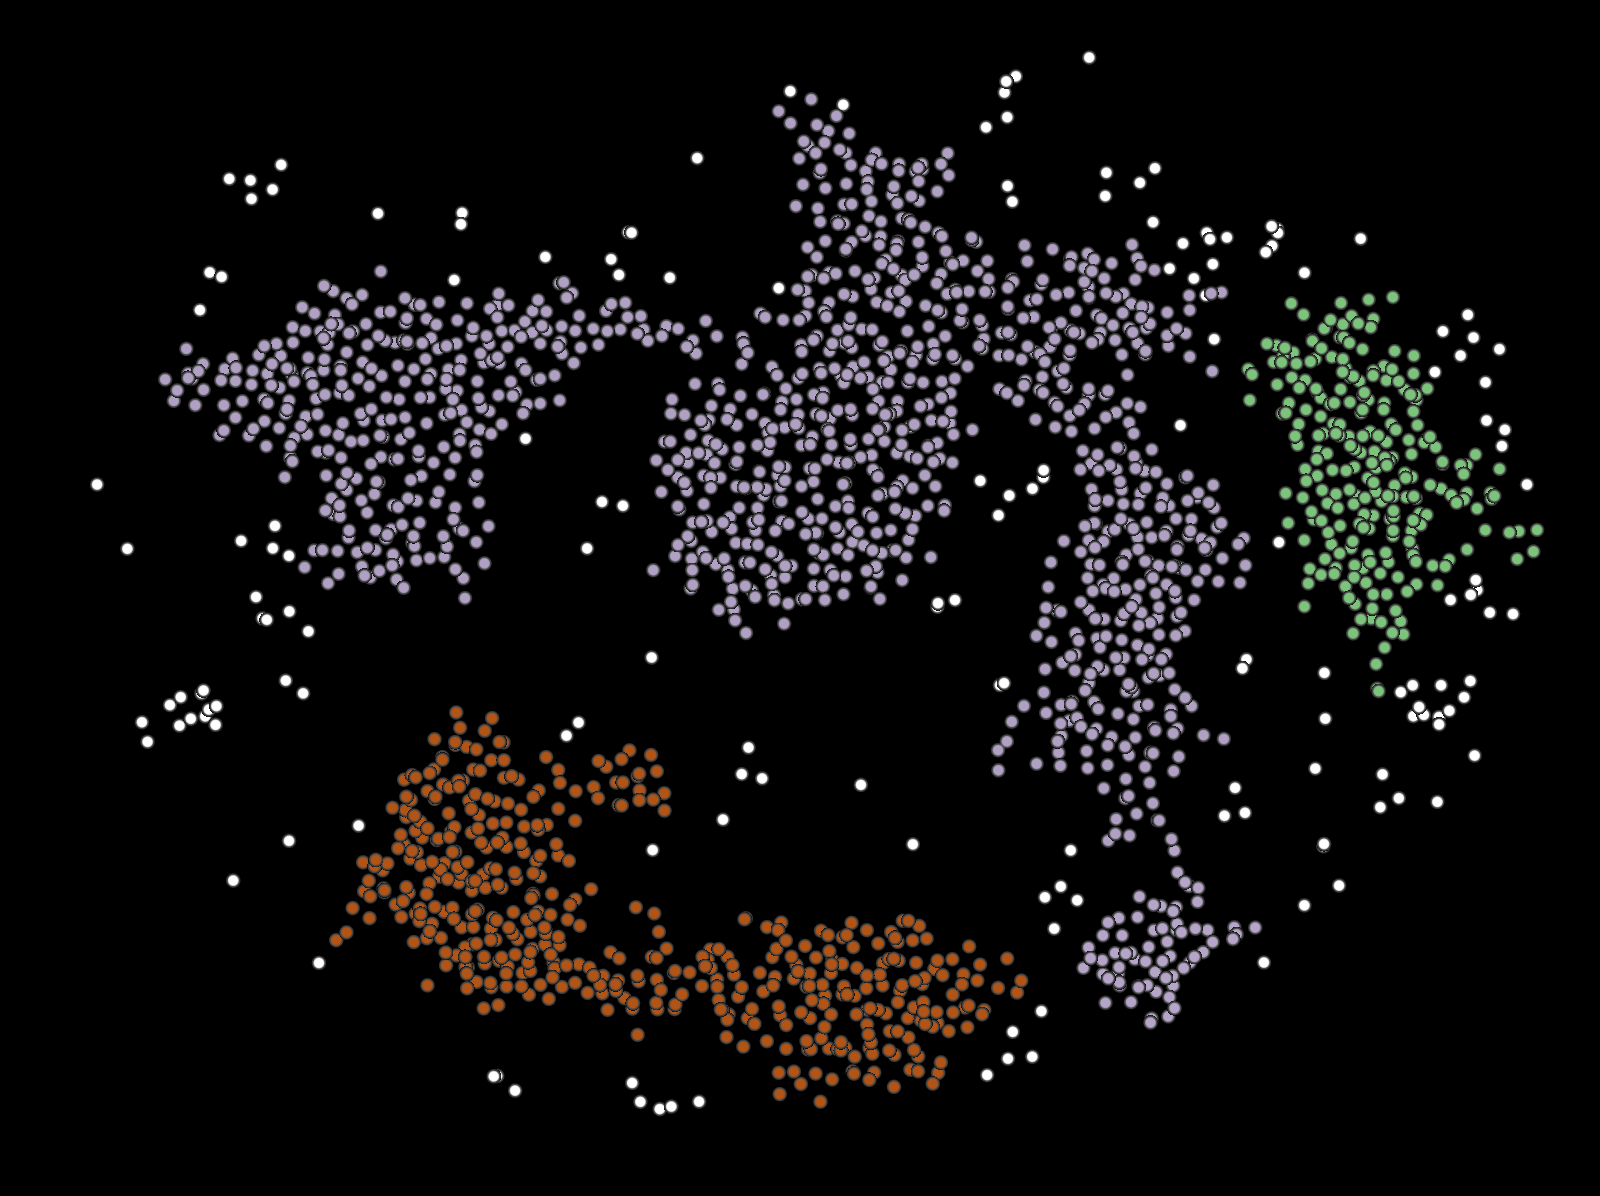
\includegraphics[width=0.32\linewidth]{figures/exp-clusters-1-only.png}
    \hfill
    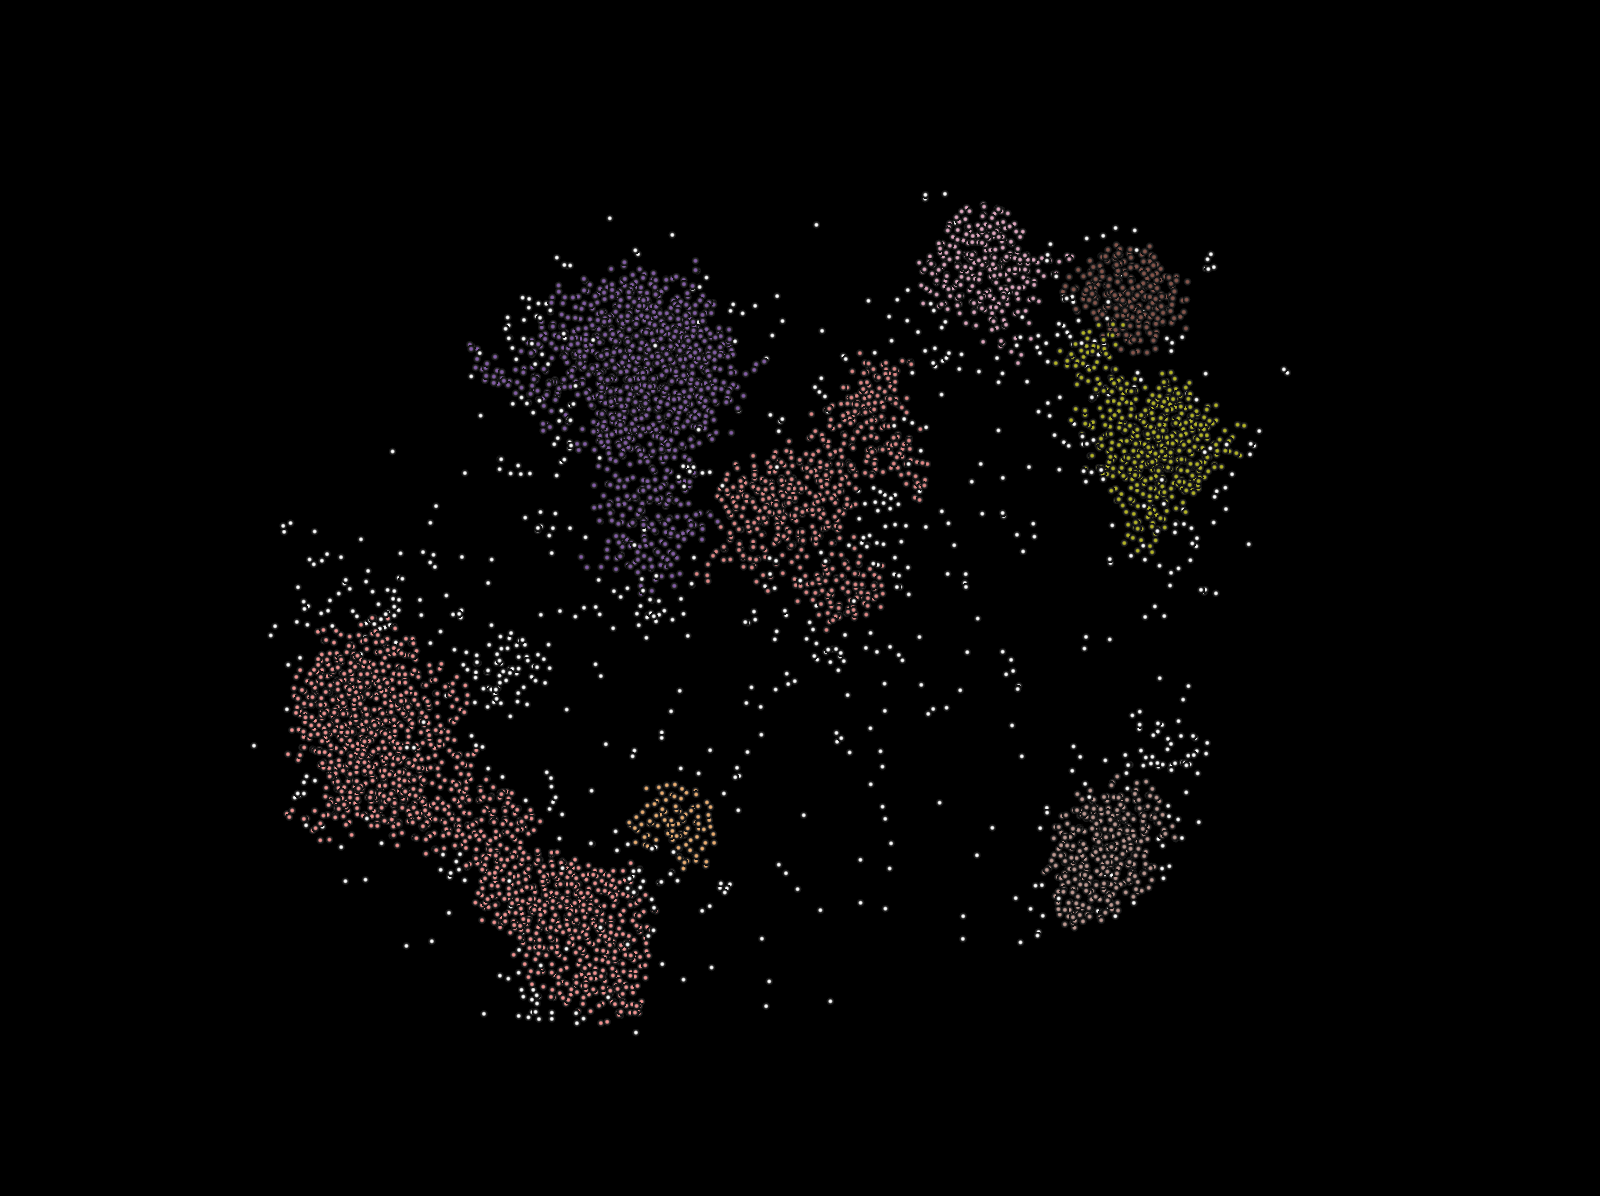
\includegraphics[width=0.32\linewidth]{figures/exp-clusters-2-only.png}
    \hfill
    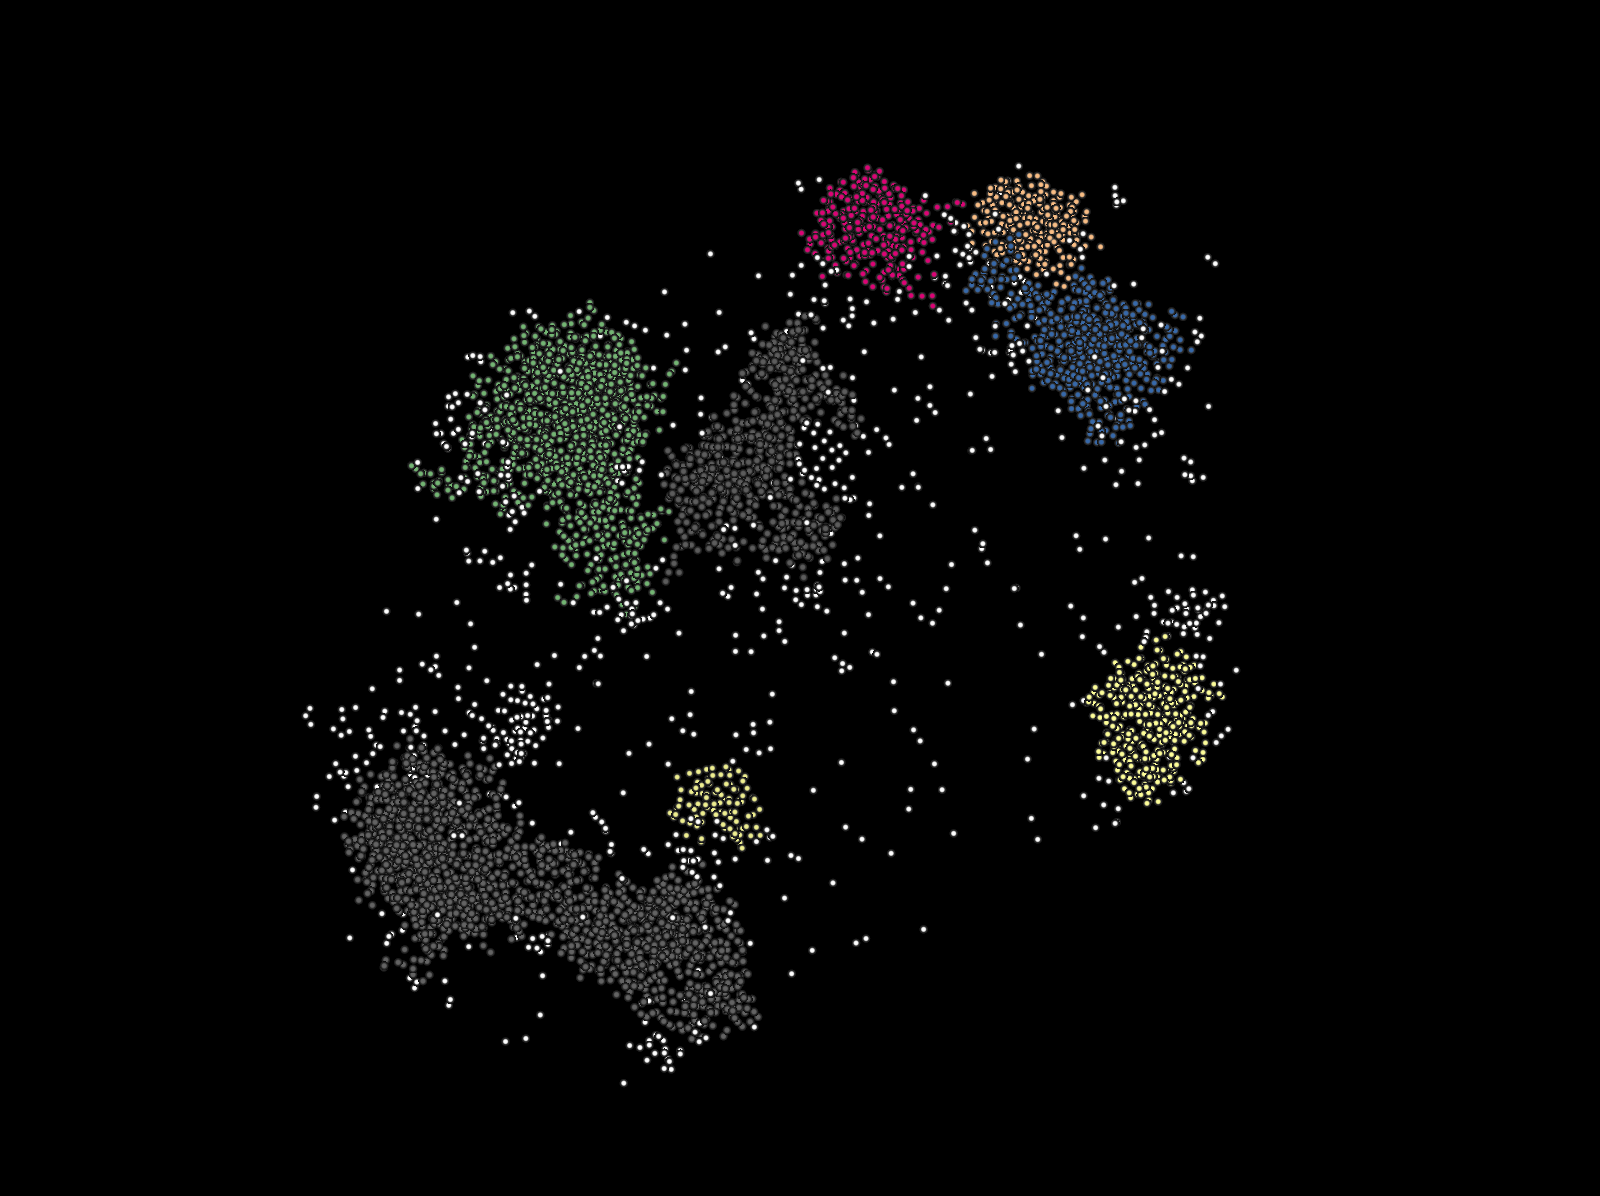
\includegraphics[width=0.32\linewidth]{figures/exp-clusters-3-only.png}
    \caption{
        Spatial cluster quantification on three experimental aggregates.
        Top: all cells, coloured by the cluster they are assigned to.
        Bottom: only the cells assigned to clusters.}
    \label{fig:exp-clusters}
\end{figure}

\begin{figure}[h]
    \centering
    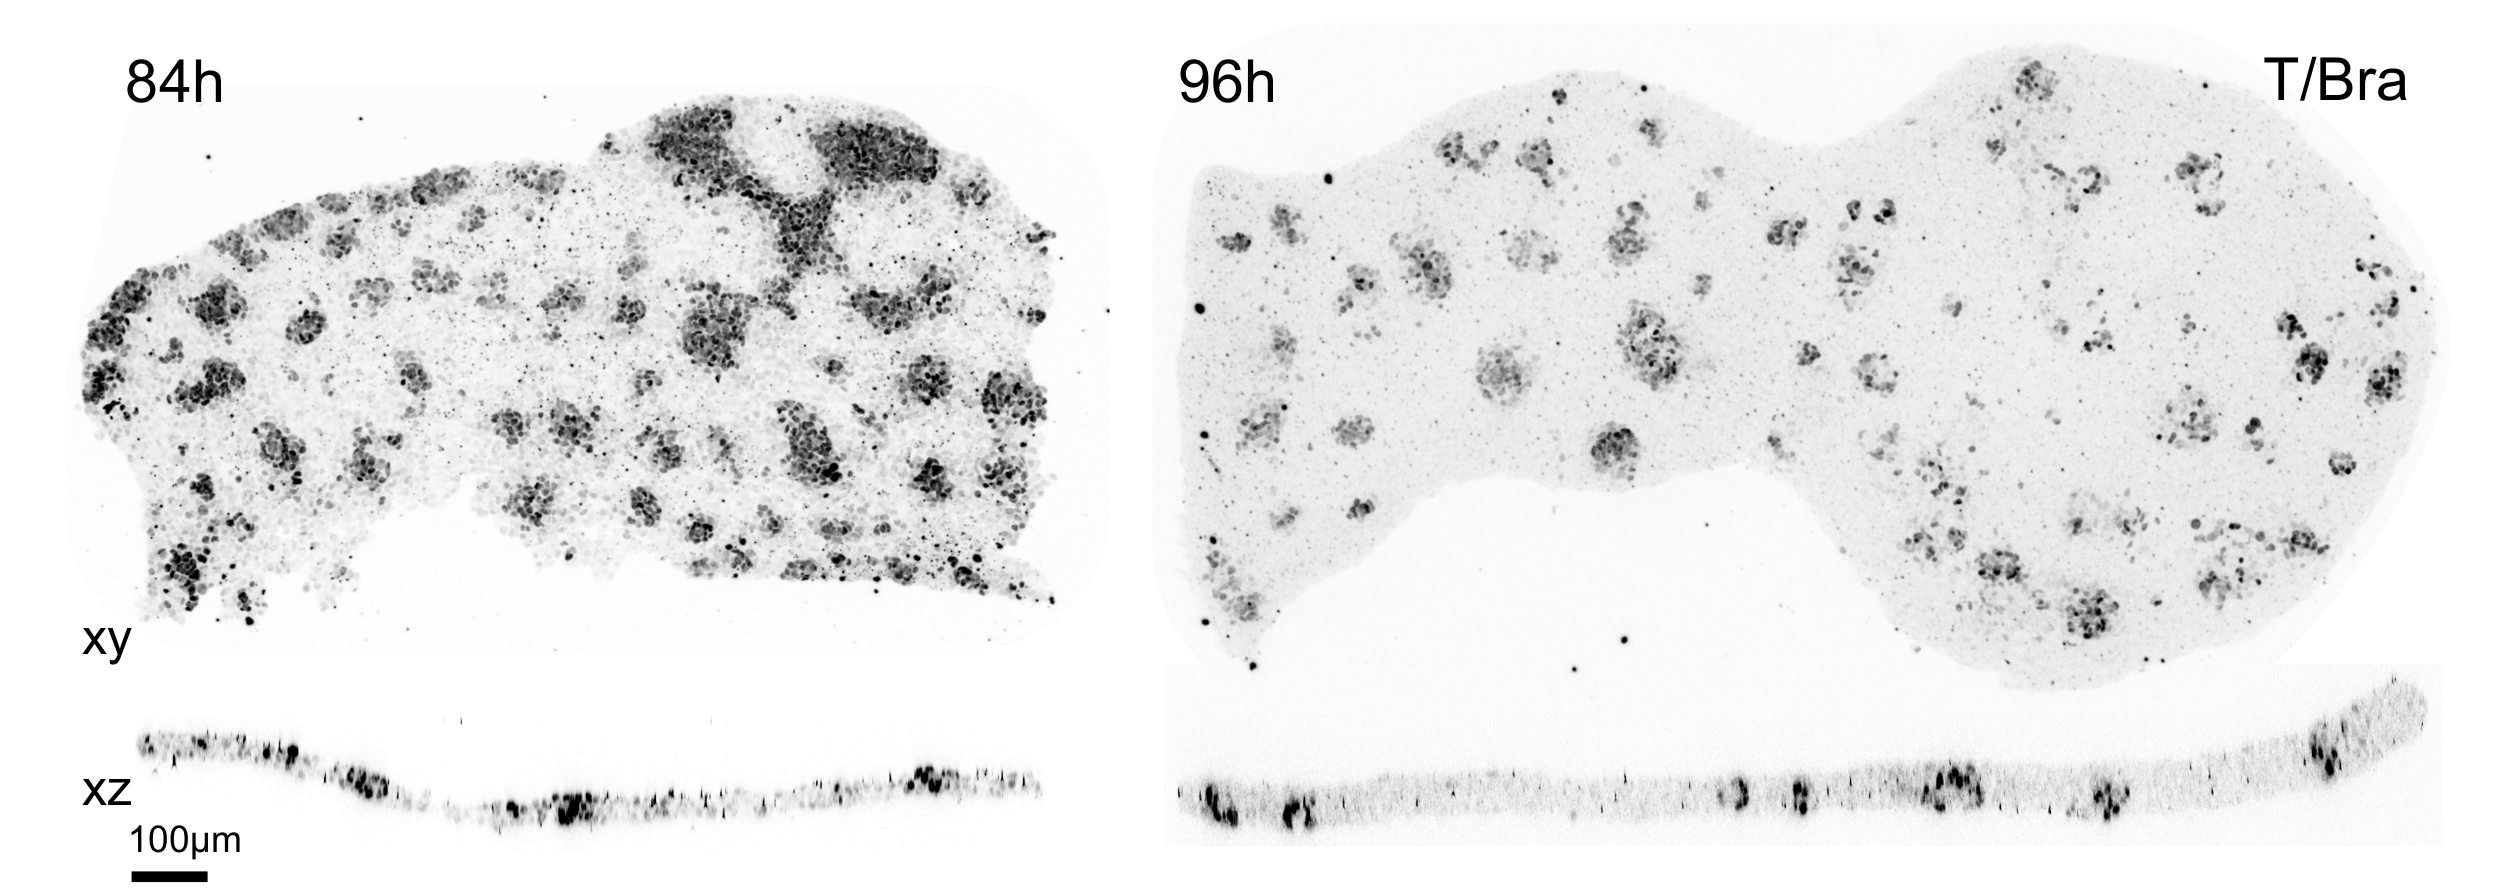
\includegraphics[width=0.9\linewidth]{figures/exp-extreme-confinement.png}
    \caption{
        T/Bra clusters in gastruloids under extreme confinement at 84\,h and 96\,h (preliminary data), seen from the top (xy) and from the side (xz).
        From V.~Weichselberger's poster.}
    \label{fig:exp-extreme-confinement}
\end{figure}


\paragraph{Polarisation.}

Polarisation is defined as follows. Let $r$ be the center of mass of the aggregate, namely $r = \frac{1}{N} \sum r_i$. Let $r_c$ be the center of mass of the centroid. Let R be the half of the length of the PC1 axis (longest axis). Then polarisation $P$ is given by 
\begin{equation*}
    P = \frac{|r - r_c|}{R}
\end{equation*}
The cutoff is set to 0.3. To determine it we just looked at the polarisation histogram of control gastruloids. Here is a plot with samples of different sizes. Where you a see that the polarisation degree at that timepoint seems to be also size dependent, but 0.3 includes the majority. 

\begin{figure}[h]
    \centering
    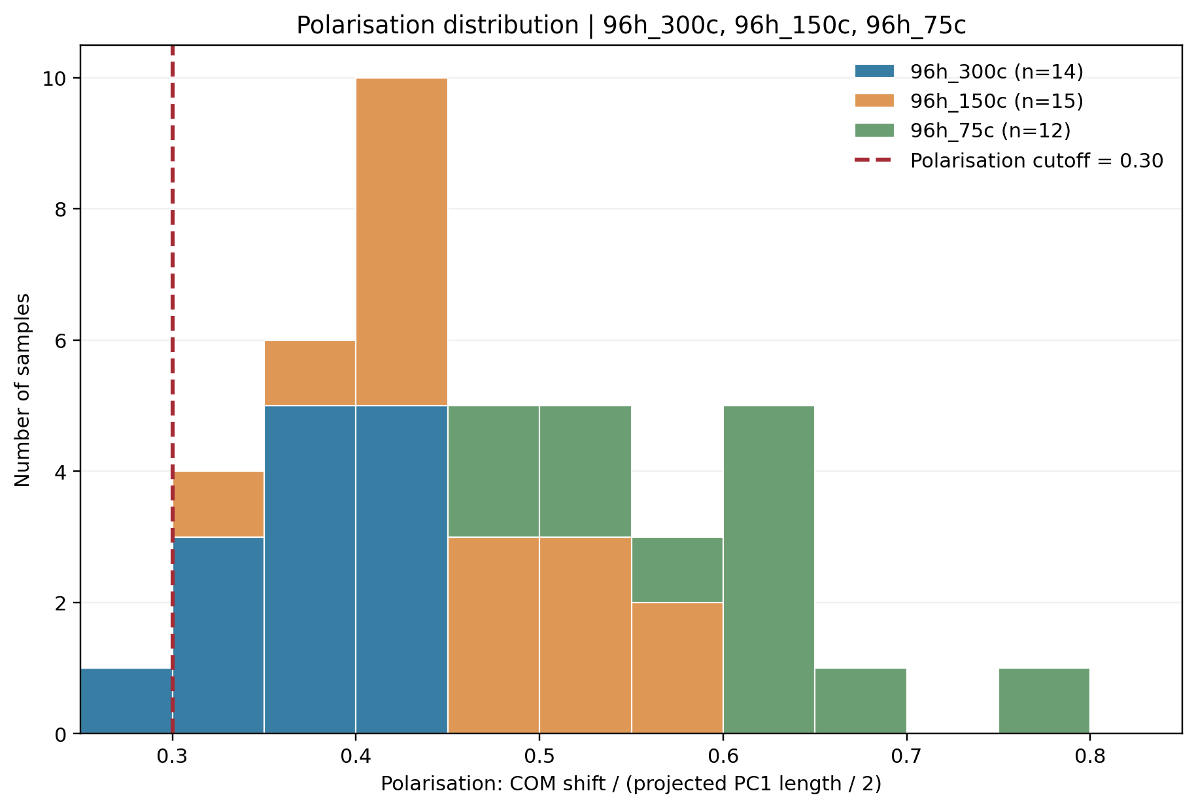
\includegraphics[height=8em]{figures/pol-histogram-1.png}

    \vspace{1em}
    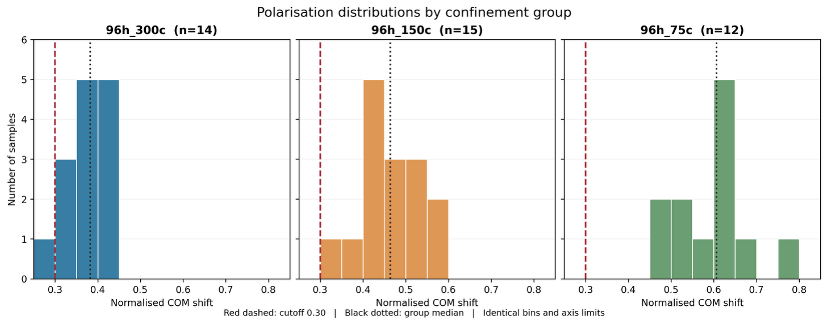
\includegraphics[height=9.5em]{figures/pol-histogram-2.png}
    \caption{
        Polarisation histogram of control gastruloids.}
    \label{fig:pol-histogramm}
\end{figure}



\FloatBarrier
\section{The physical description}

\subsection{Simplificating reality}

First, we grow and differentiate a gastruloid aggregate before polarisation begins. Instead of the three-state description used in \cite{oriola} ($A\to B\to C$), we assume all $A$ cells have differentiated away at the moment of squeezing and therefore only consider $B$ ($T^+$) and $C$ ($T^-$) cells. 

We define out initial aggregate to be a spheroid with a central cluster of $B$ cells containing about $60\%$ of the cells in the aggregate. The rest of the cells are in state $C$. If we were to let this further evolve, this cluster would polarise.

In order to model the behaviour of the confined aggregate, we won't study the confinement process but instead consider an already-squeezed aggregate with a $B$-centroid. We define it by growing an aggregate under confinement, setting the inital cells as they would result on confining the spherical gastruloid, letting the cells relax, and then starting differentiaion and proliferaiton.

We want to replicate all three behaviours described previously. 

\paragraph{Fusion.} We use fusion as a sanity check to see that they are not only replicating the confined patterning, just like we do with unconfined polarisation. We see that, under certain conditions, two modelled gasruloids fuse as they do experimentally. In particular, we see that
\begin{enumerate}
    \item Two spherical $B$-only aggregates fuse perfectly forming a single sphere.
    \item A $B$-aggregate and a $C$-aggregate glue together but do not form a single sphere.
\end{enumerate}

\begin{figure}[h]
    \centering
    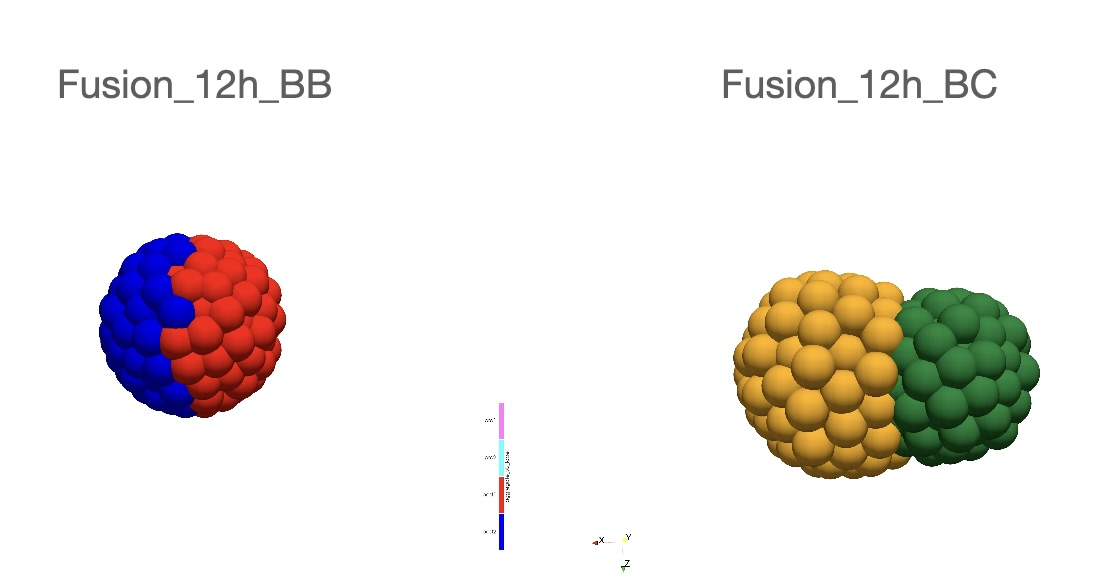
\includegraphics[height=8em]{figures/fusions-relevant.jpeg}
    \caption{
        Expected fusion behaviour.}
    \label{fig:expected-fusion}
\end{figure}


\subsection{Modelling 3D aggregates}

\paragraph{Mechanics.}

    In the agent-based simulations, a single cell $i$ is represented by the position of its centre of mass $\mathbf{x}_i$ and its dynamics is given by the following overdamped equations of motion:
    \begin{align*}
        \dot{\mathbf{x}}_i &= \mathbf{v}_i \,,\\
        {\mathbf{v}}_i &= \frac{1}{{\lambda} n_i} \sum_j {\mathbf{F}}_{ij} + \frac{\alpha}{n_i} \sum_j {\mathbf{v}}_j \,.
    \end{align*}
    where isotropic friction forces are assumed and $\mathbf{v}_i$ is the cell velocity. $\lambda_s$ is the friction coefficient for the cell-substrate or cell-ECM interaction, while $\lambda_r$ is the relative cell-cell friction coefficient.

    The passive force $\mathbf{F}_{ij}$ describes cell-cell adhesion and repulsion that depends on the position of the two interacting cells $(i,j)$ as well as their states $(s_i,s_j)\in\{B,C\}^2$:
    \begin{equation*}
        \mathbf{F}_{ij}(s_i, s_j, d_{ij}) =
        \begin{cases}
            f(d_{ij})\, \hat{\mathbf{r}}_{ij} 
                F_\text{rep}^{(s_i, s_j)}, & \text{if } d_{ij} \leq 2r \\
            f(d_{ij})\, \hat{\mathbf{r}}_{ij} 
                F_\text{att}^{(s_i, s_j)}, & \text{if } 2r < d_{ij} < 2\mu r \\
            0, & \text{otherwise} \,,
        \end{cases}
    \end{equation*}
    where $F^{(s_i,s_j)}_{\text{rep}}$, $F^{(s_i,s_j)}_{\text{adh}}$ are $3 \times 3$ matrices that describe the magnitude of the interaction,
    ${d}_{ij} = {|\mathbf{x}_i - \mathbf{x}_j|}$,
    $\hat{\mathbf{r}}_{ij} = \frac{\mathbf{x}_i - \mathbf{x}_j}{d_{ij}}$,
    and
    \begin{equation*}
        f(d_{ij}) = \left(\frac{2r}{d_{ij}} - 1\right)\left(\frac{2\mu r}{d_{ij}} - 1\right) \,.
    \end{equation*}

    \begin{remark}
        In the code we set $\hat\alpha=\lambda\alpha$ and so
        \begin{equation*}
            {\mathbf{v}}_i = \frac{1}{{\lambda} n_i}\left( \sum_j {\mathbf{F}}_{ij} + \alpha \sum_j {\mathbf{v}}_j \right) \,.
        \end{equation*}
    \end{remark}

\paragraph{Division.}

    Cells undergo division according to the following rules:
    \begin{itemize}
        \item A division axis is randomly chosen over the unit sphere.
        \item The two daughter cells are generated with equal radius as the parent cell and positioned on opposite sides of the division axis which is centred at the parent cell's location. The daughter cells are generated with their centre of mass at a fixed distance from that of the parent cell.
        \item A new division time is then assigned to each daughter cell, sampled from
        \begin{equation*}
            \mathcal{U}\big(\tau_{\text{div}}(1 - \sigma_{\text{div}}),\ \tau_{\text{div}}(1 + \sigma_{\text{div}})\big),
        \end{equation*}
    \end{itemize}

\paragraph{Differentiaton.}

    The {transition rate} from $B$ to $C$ is constant,
    \begin{equation*}
        r_{B\rightarrow C} \equiv q \,,
    \end{equation*}
    so every $B$ cell becomes $C$ with probability $q\,\Delta t$ per time step.

    \begin{remark}
        The fraction of $B$ cells falls from $60\%$ to $20\%$ in about 21 hours, against 24 hours (from 72 to 96 h) in the experiments.
    \end{remark}

\paragraph{Confinement.}
    The {plates} sit at $z=0$ and $z=L$, with $L = 2.1\,r \times$ (number of layers). They are rigid: a cell touching a plate cannot move further into it, so the slab keeps its thickness during the whole simulation. A cell closer than $0.05$ to a plate also feels {plate friction}, an extra in-plane drag:
    \begin{equation*}
        \big(\lambda n_i\, \mathbb{I} + \lambda_\text{wall}\, \mathbb{P}\big)\, \mathbf{v}_i = \sum_j \mathbf{F}_{ij} + \alpha \sum_j \mathbf{v}_j \,, \qquad \mathbb{P} = \mathbb{I} - \hat{\mathbf{z}}\hat{\mathbf{z}}^\top \,,
    \end{equation*}
    where $\mathbb{P}$ projects onto the $xy$-plane, so the extra drag acts only parallel to the plates.

    This plate friction stands for adhesion to, or rubbing on, the confining surfaces.


\subsection{Analysis of the model}

\begin{remark}
    Pulling two attached cells apart costs the \textbf{adhesion energy}
    \begin{equation*}
        W_{XY} = \int_{2r}^{2\mu r} |F|\,\diff d = F_\text{att}^{(X,Y)}\, 2r\, A(\mu_{XY}) \,, \qquad A(\mu) = (1+\mu)\ln\mu - 2(\mu - 1) \,.
    \end{equation*}
    These energies set the surface tensions $\sigma_X = W_{XX}/2$ and the interfacial tension $\gamma_{BC} = (W_{BB} + W_{CC})/2 - W_{BC}$. Two aggregates glue without rounding into one sphere when $|\sigma_B - \sigma_C| < \gamma_{BC} < \sigma_B + \sigma_C$.
\end{remark}



\section{The simulations}

The main challenge of the simulations is to replicate all the aforementioned behaviours using the same model. All the parameters are in Table~\ref{parameters}. All the figures are three-dimensional; a top view leaves out the cells above the mid-plane, since the outer $C$ cells would hide the $B$ pattern otherwise.

\subsection{Initial condition}

Figure~\ref{initial-condition} shows the initial aggregate.

\begin{figure}[h]
    \centering
    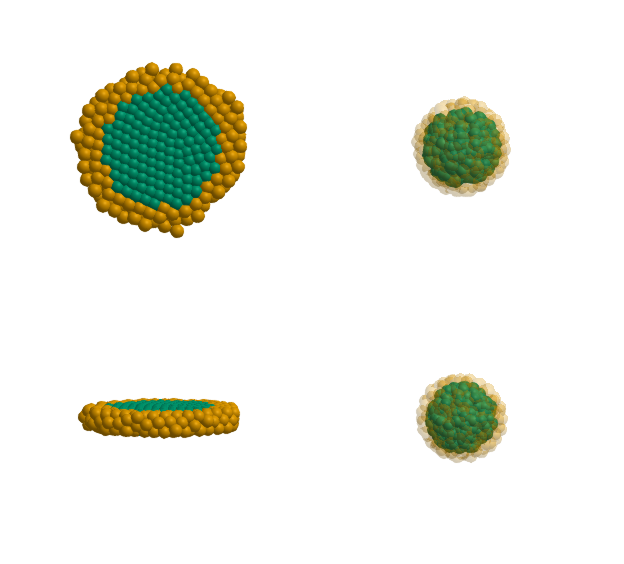
\includegraphics[width=0.8\linewidth]{figures/fig1_initial_condition.png}
    \caption{Initial condition: a  $B$-centroid containing $60\%$ of the cells in the aggregate; the rest are $C$. Left: 2 layers, top view cut at the mid-plane; right: unconfined, whole aggregate with $C$ translucent; both $N_0=600$, drawn at the same scale, at the start of differentiation ($t = 0$).}
    \label{initial-condition}
\end{figure}

\subsection{Fusion}

We place two aggregates close in space and let the mechanics evolve, without division nor differentiation (see Figure~\ref{fusion}). The $BB$ and $CC$ cases fuse, whereas $BC$ glues.

\begin{figure}[htbp]
    \centering
    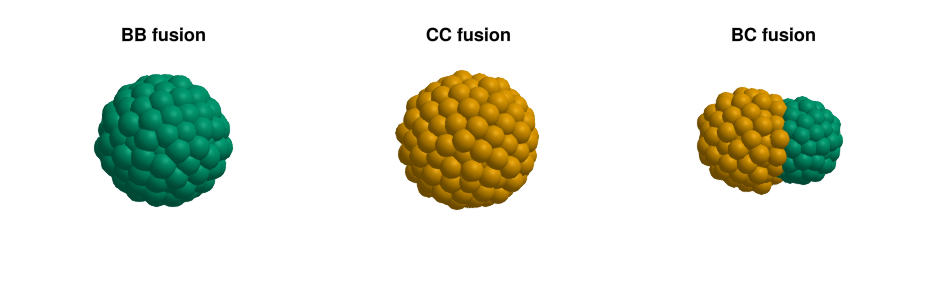
\includegraphics[width=0.75\linewidth]{figures/fig5_fusion.png}
    \caption{Fusion assay after 24 hours: $BB$, $CC$ and $BC$ doublets.}
    \label{fusion}
\end{figure}

\subsection{Polarisation}

Unconfined aggregates of up to $N_0 = 600$ cells polarise before $B$ runs out (Figure~\ref{polarisation}). Larger aggregates ($N_0 = 1200$ to $4800$) still have a central cluster when $20\%$ of the cells are $B$, and the largest never polarise.

\begin{figure}[htbp]
    \centering
    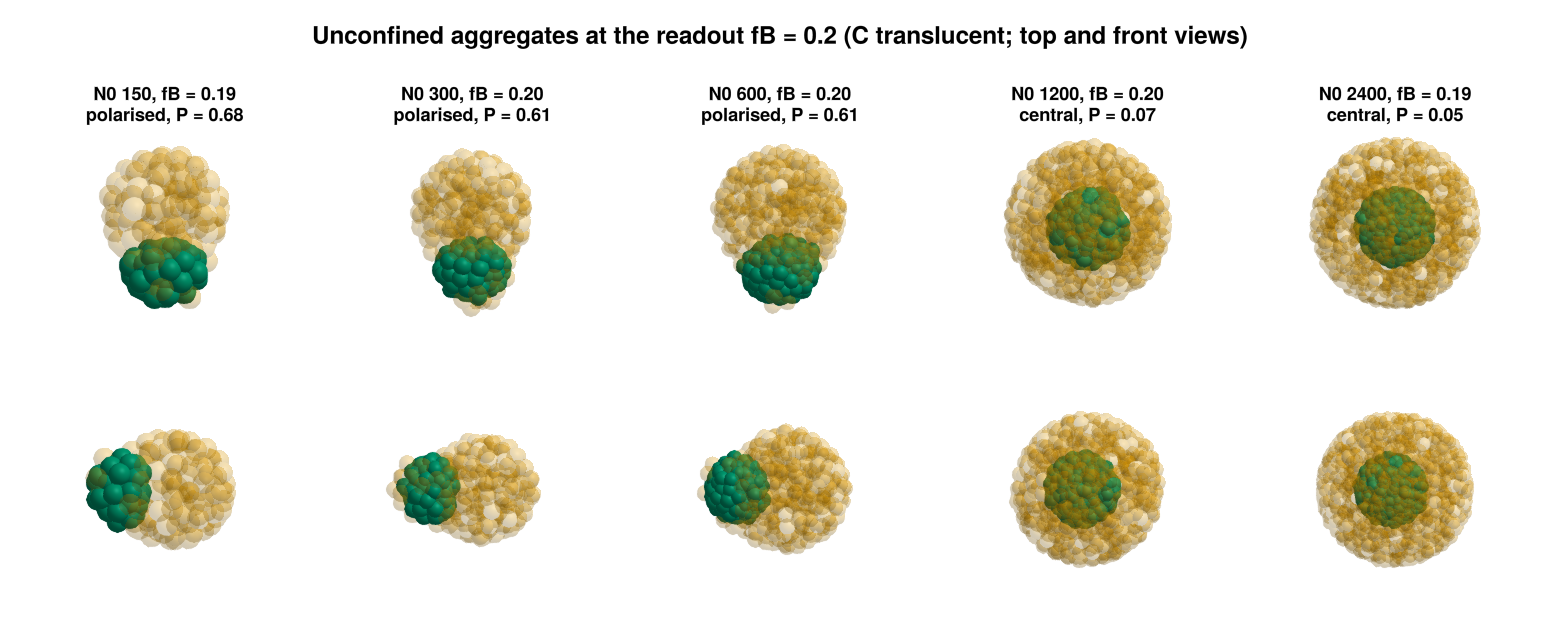
\includegraphics[width=\linewidth]{figures/fig4_unconfined.png}
    \caption{Unconfined aggregates of $N_0 = 150$ to $2400$ cells when $20\%$ of the cells are $B$ (17 to 19~h after the start of differentiation). Top and front views of the whole aggregate, $C$ translucent. Rotated so that $B$ points to the right.}
    \label{polarisation}
\end{figure}

\subsection{Confinement}

Figure~\ref{behaviours} follows the same aggregate under no, medium and strong confinement. Figure~\ref{patterns} shows patterns from one to four layers.

\begin{figure}[htbp]
    \centering
    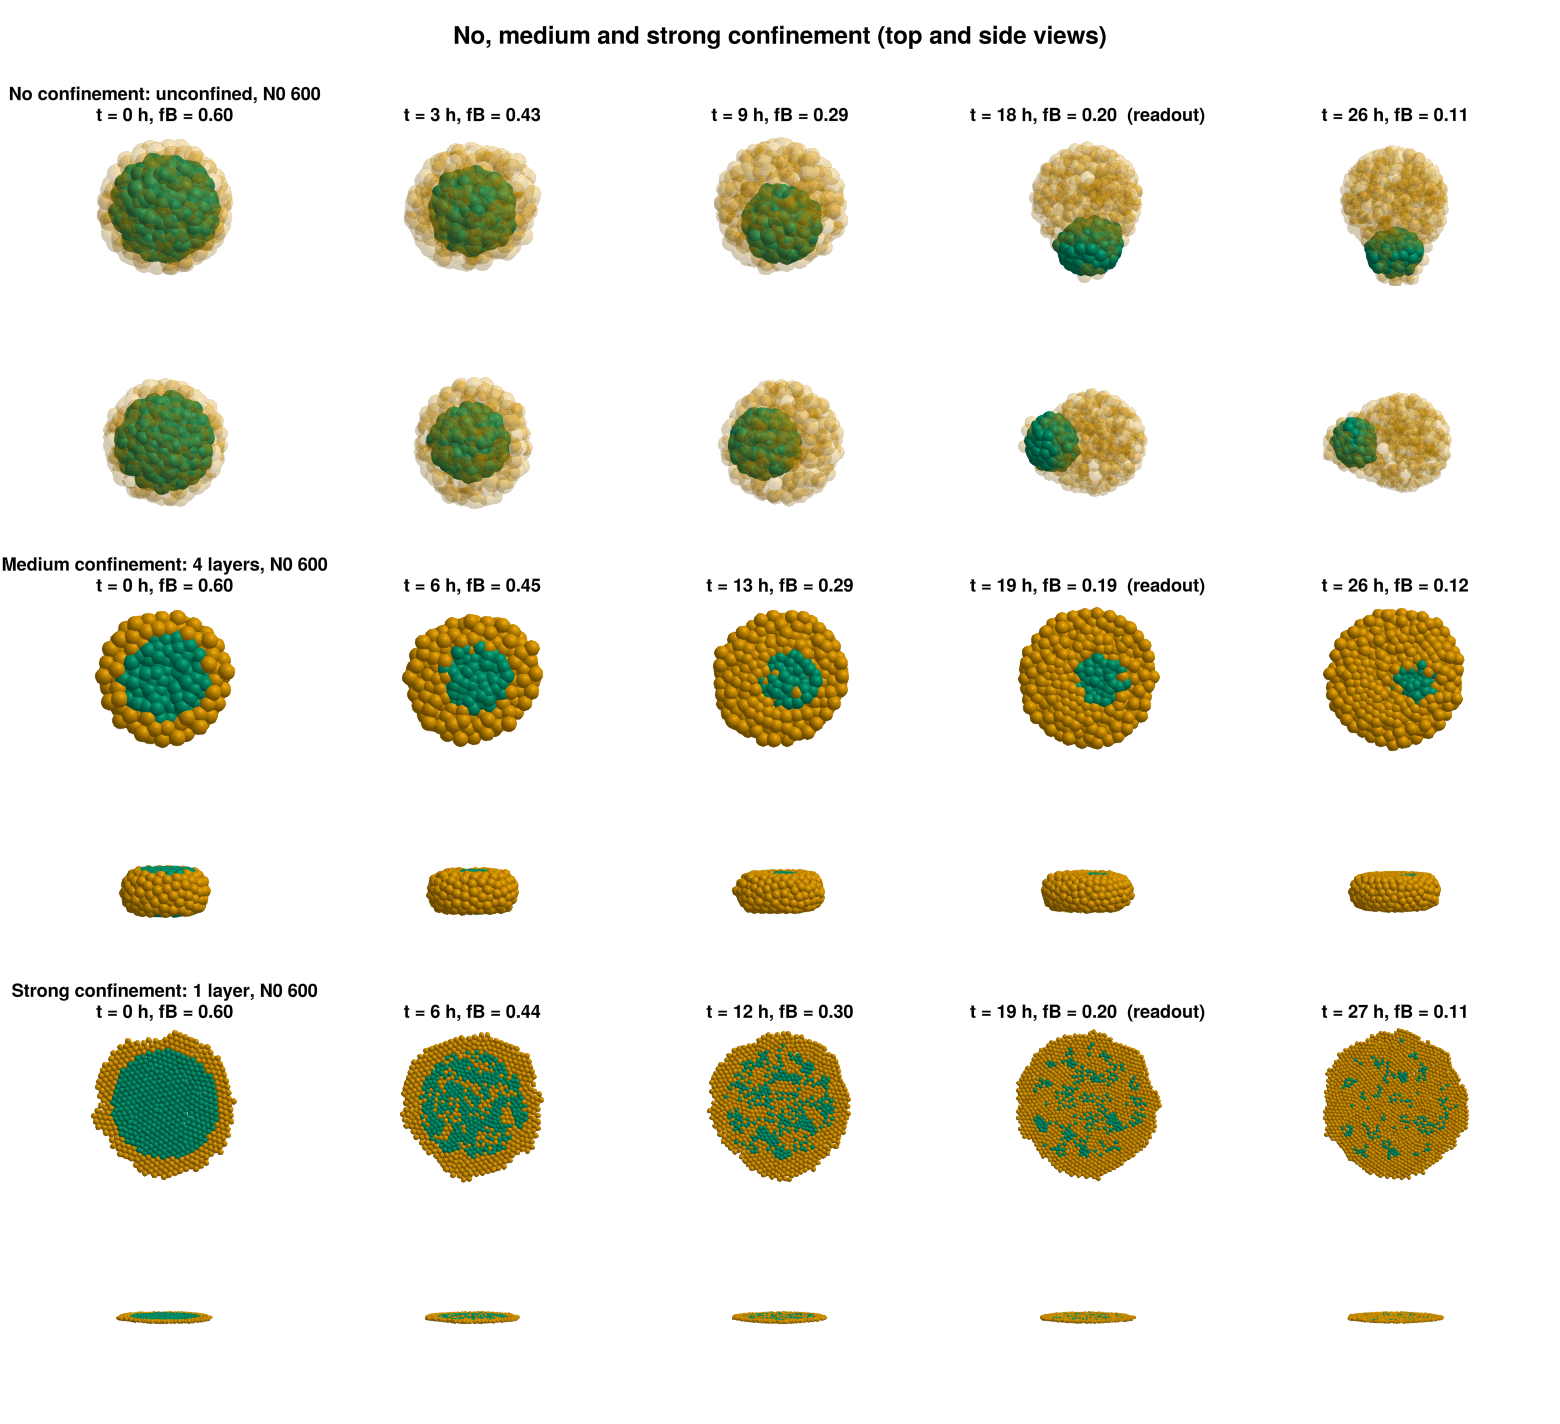
\includegraphics[width=\linewidth]{figures/fig2_behaviours.png}
    \caption{$N_0=600$ cells with no confinement (polarises), 4 layers (central cluster that differentiates away) and 1 layer (islands), from the start of differentiation ($0$~h) to $12\%$ of $B$ cells ($26$--$27$~h). The readout is at $20\%$ ($18$--$19$~h). Confined: top view cut at the mid-plane; unconfined: whole aggregate, $C$ translucent.}
    \label{behaviours}
\end{figure}

\begin{figure}[htbp]
    \centering
    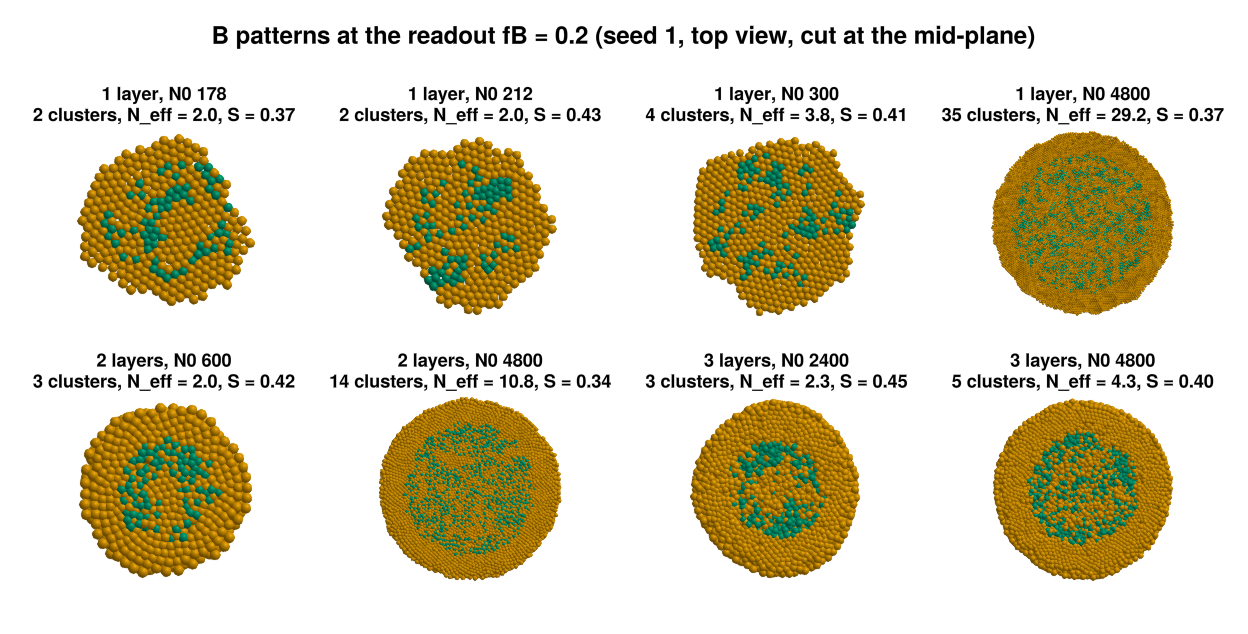
\includegraphics[width=\linewidth]{figures/fig3_patterns.png}
    \caption{Patterns when $20\%$ of the cells are $B$ (the readout, $11$ to $24$~h after the start of differentiation depending on the run, $18$~h on average), from one to three layers. Top view cut at the mid-plane.}
    \label{patterns}
\end{figure}

In thick slabs the pattern starts as a ring: the core hollows out and then breaks into islands (Figure~\ref{ring}).

\begin{figure}[htbp]
    \centering
    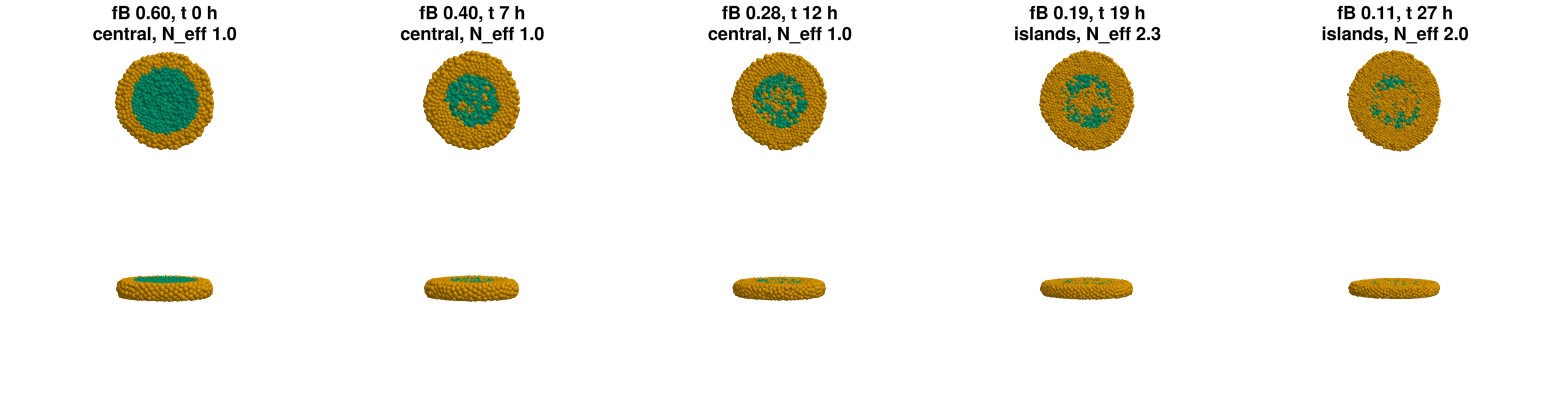
\includegraphics[width=\linewidth]{figures/ring-3layers.png}
    \caption{Three layers, $N_0 = 2400$: the central cluster hollows into a ring, which breaks into islands, from the start of differentiation to $27$~h. Top: cut at the mid-plane; bottom: side view.}
    \label{ring}
\end{figure}

\subsection{Patterns in thick slabs}

With the parameters of early October, every slab of three or more layers ended as one compact central cluster, at any $N_0$ up to 4800. Table~\ref{attempts} lists what we tried at three layers and $N_0 = 2400$. The salt-and-pepper start is the one the July runs used: $75\%$ $B$, $15\%$ $A$ and $10\%$ $C$, shuffled inside the core.

\begin{table}[htbp]
    \centering
    {\small
    \begin{tabular}{lll}
        \hline
        \textbf{Change} & \textbf{Outcome} & \textbf{Looseness $S$} \\
        \hline
        $B$ fraction $65\%$ instead of $60\%$ & central & 0.88 \\
        $B$ cells scattered outside the core ($10$ to $30\%$ of them) & central & 0.86--0.89 \\
        $C$ cells mixed into the core ($10$ to $30\%$ of it, as in July) & central & 0.89--0.91 \\
        Spring plates (July) instead of rigid ones & central & 0.91 \\
        Plate friction 5 instead of 1.5 & central & 0.89 \\
        July mechanics ($F_\text{rep}^{BB}=3$, $F_\text{rep}^{CC}=5.1$) & central & 0.90--0.93 \\
        $F_\text{att}^{CC}$: $3 \to 3.6$ & central & 0.88 \\
        $F_\text{att}^{BB}$: $6.4 \to 5.6$ & central, looser & 0.72 \\
        $\lambda$ multiplied by 2, 3 or 4 & central (and no polarisation) & 0.52--0.84 \\
        $\mu_{BB}$: $2 \to 1.85$ or $1.8$ & $B$ dissolves into $C$ & 0.30--0.35 \\
        $\boldsymbol{\mu_{BB}}\colon \mathbf{2 \to 1.9}$ & \textbf{ring, then islands} & \textbf{0.45} \\
        \hline
    \end{tabular}
    }
    \caption{What we tried to obtain patterns at three layers ($N_0 = 2400$). $S$ is about $0.9$ for a compact cluster and $0.4$--$0.6$ for loose patterns.}
    \label{attempts}
\end{table}

What changes the outcome is the cohesion of the $B$ tissue. In a slab of one or two layers, the $C$ cells that appear inside the $B$ core cannot get out, since cells cannot pass each other, and they split the core. From three layers on, cells pass over and under each other, and a cohesive $B$ core squeezes the new $C$ cells out and stays as one cluster. Shortening the $B$--$B$ attraction range from $\mu_{BB}=2$ to $1.9$ lowers the $B$--$B$ adhesion energy from $W_{BB}=1.02$ to $0.79$, still above $W_{CC}=0.65$. Then small cores stay compact, but a large core in a thick slab opens into a ring. It is the energy and not the range: with $\mu_{BB} = 1.8$ and $F_\text{att}^{BB}$ raised to keep $W_{BB} = 1.02$, the core stays compact. At $\mu_{BB} = 1.85$ ($W_{BB} \approx W_{CC}$), $B$ is no longer more cohesive than $C$ and simply dissolves into it, even in small aggregates (Figure~\ref{dissolves}).

\begin{figure}[htbp]
    \centering
    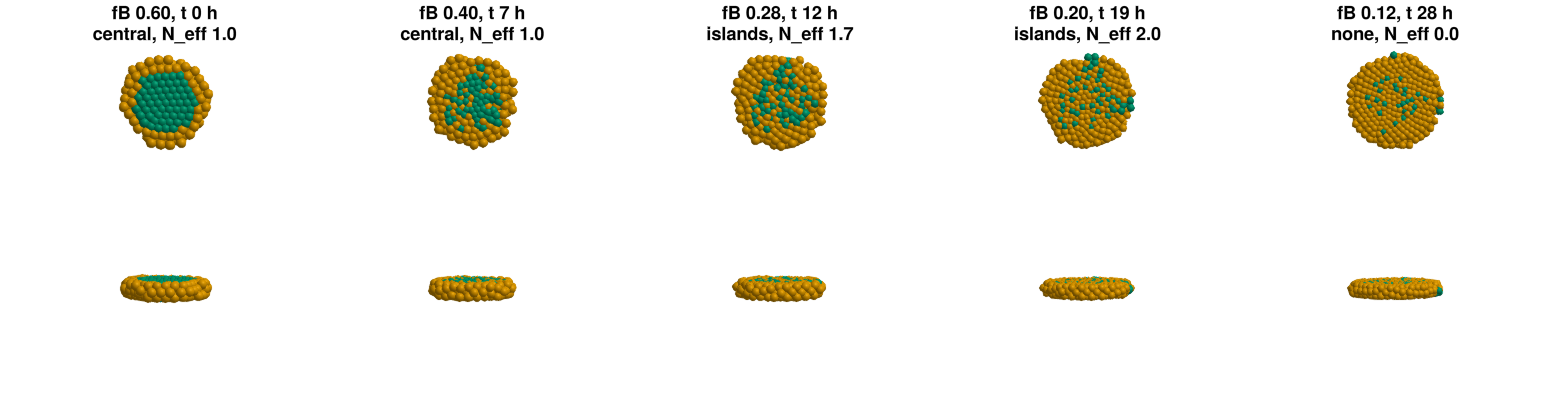
\includegraphics[width=\linewidth]{figures/dissolves-muBB1.8.png}
    \caption{With $\mu_{BB}=1.8$ the $B$ cells dissolve into the $C$ tissue (2 layers, $N_0 = 300$), from the start of differentiation to $28$~h.}
    \label{dissolves}
\end{figure}

The new parameter set keeps the other behaviours: small squeezed aggregates keep a central cluster, monolayers give sparse islands, unconfined aggregates polarise, and $BC$ fusion glues.

\subsection{Reading the outcome}

The outcome is read from the positions $\mathbf{x}_i$ and states $s_i$ of the cells when $20\%$ of them are $B$, with the experiments' clustering and polarisation (see \emph{The experiment}), adapted to the size of our aggregates.

\paragraph{Clusters.} Let $\rho = 2.6\,r = 13~\mu$m and let $\mathcal{N}_i = \{\, j \neq i : |\mathbf{x}_i - \mathbf{x}_j| \le \rho \,\}$ be the neighbours of cell $i$. A $B$ cell is a \emph{core} cell if at least a fraction $\phi$ of its neighbours are $B$:
\begin{equation*}
    i \in \mathcal{K} \iff s_i = B, \quad \mathcal{N}_i \neq \emptyset \quad \text{and} \quad \big|\{\, j \in \mathcal{N}_i : s_j = B \,\}\big| \ \ge\ \phi\, |\mathcal{N}_i| .
\end{equation*}
Two core cells are linked if $|\mathbf{x}_i - \mathbf{x}_j| \le \rho$, and the clusters are the connected components of the graph of core cells with these links. Every other $B$ cell with a core cell within $\rho$ joins the cluster of its nearest core cell (a \emph{border} cell); the remaining $B$ cells belong to no cluster. Clusters of fewer than $n_\text{min}$ cells (core and border) are discarded. If $n_1, \dots, n_K$ are the sizes of the clusters kept and $p_k = n_k / \sum_l n_l$, the effective number of clusters is
\begin{equation*}
    N_\text{eff} = \frac{1}{\sum_{k=1}^K p_k^2} ,
\end{equation*}
which is $K$ when the clusters have the same size and close to $1$ when one of them holds most of the cells.

\paragraph{Polarisation.} With $\bar{\mathbf{x}} = \frac1N \sum_i \mathbf{x}_i$ the centre of mass of the aggregate and $\bar{\mathbf{x}}_B$ that of the $B$ cells, let $\mathbf{e}_1$ be the first principal axis of the cell positions (the leading eigenvector of $\frac1N\sum_i (\mathbf{x}_i - \bar{\mathbf{x}})(\mathbf{x}_i - \bar{\mathbf{x}})^\top$) and $u_i = (\mathbf{x}_i - \bar{\mathbf{x}})\cdot\mathbf{e}_1$. Then
\begin{equation*}
    P = \frac{|\bar{\mathbf{x}}_B - \bar{\mathbf{x}}|}{R}, \qquad R = \tfrac12\big(\max_i u_i - \min_i u_i\big) .
\end{equation*}

\paragraph{Outcome.} In this order:
\begin{enumerate}
    \item \emph{other}, if no cluster is kept ($K = 0$);
    \item \emph{Polarisation}, if $P \ge 0.3$;
    \item \emph{Clusters}, if $N_\text{eff} \ge 1.5$;
    \item \emph{B-centroid} otherwise: one dominant cluster that has not moved. A ring that has not broken is a $B$-centroid, as in the experiments' medium confinement.
\end{enumerate}

\paragraph{Differences with the experiments.} We keep clusters of $n_\text{min} = 10$ cells instead of $20$, because our aggregates are $10$ to $100$ times smaller (with $20$, monolayers of up to $300$ cells have no cluster at all). A core cell needs half of its neighbours to be $B$ ($\phi = 0.5$) instead of $40\%$ ($\phi = 0.4$): with $40\%$, a ring whose pieces still touch through threads of one or two $B$ cells is one cluster, and with $50\%$ these threads are border cells and the pieces are separate clusters. The radius $\rho$ and the cutoffs $P \ge 0.3$ and $N_\text{eff} \ge 1.5$ are those of the experiments.

\subsection{Phase space}

Finally, we compute the phase space relating the outcome, the number of layers and the number of cells $N_0$ at the moment of squeezing (Figure~\ref{phase-space}), with 2 or 3 simulations per point (178 in total). The outcome is read when $20\%$ of the cells are $B$ (96 h in the experiments) and classified as central cluster, pattern (a ring or islands), polarised, or other.

\begin{figure}[htbp]
    \centering
    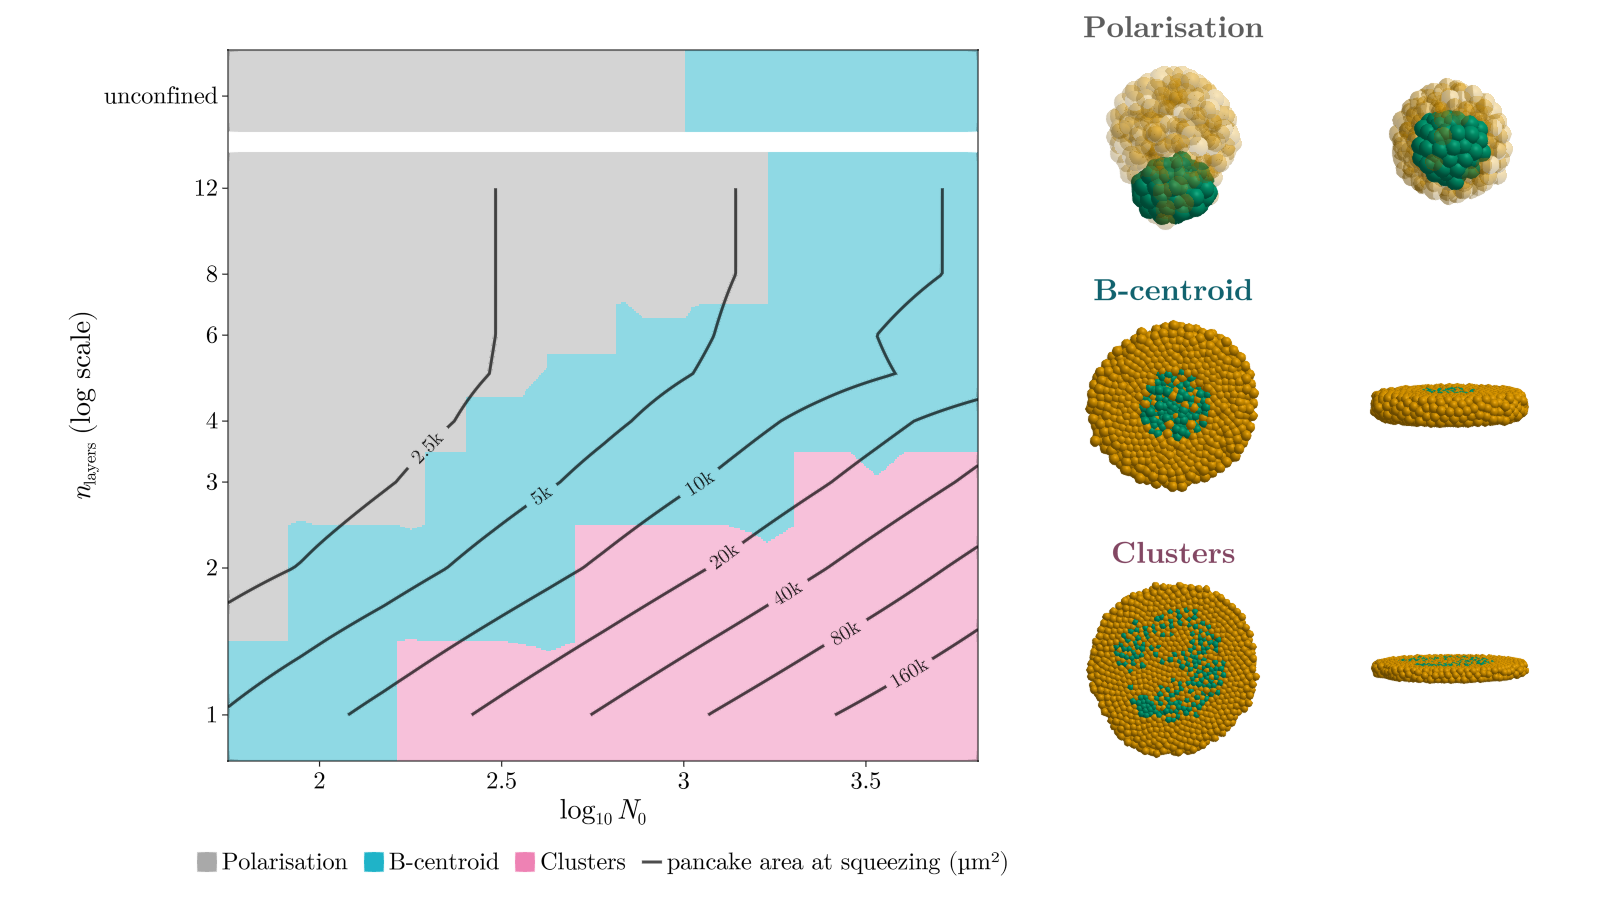
\includegraphics[width=\linewidth]{figures/phase_space.png}
    \caption{Phase space, read when $20\%$ of the cells are $B$ ($18$~h after the start of differentiation on average). The colour is the majority outcome of the nearest simulated point (a tie between seeds goes to the outcome that wins later, at $12\%$). Lines: area of the pancake at squeezing ($\mu$m$^2$). Right: one example of each outcome (8 layers, $N_0 = 300$; 3 layers, $N_0 = 1200$; 2 layers, $N_0 = 1200$).}
    \label{phase-space}
\end{figure}

\begin{table}[htbp]
    \centering
    {\small
    \begin{tabular}{cccc}
        \hline
        \textbf{Layers} & \textbf{Polarised up to $N_0$} & \textbf{Central cluster} & \textbf{Patterns from $N_0$} \\
        \hline
        1 & -- & 75--150 & $\approx 160$ \\
        2 & 75 & 89--424 & $\approx 500$ \\
        3 & 150--178 & 212--1697 & $\approx 2000$ \\
        4 & 212 & 300--4800 & none up to 4800 \\
        6--12 & 600--1200 & up to 2400 & none up to 2400 \\
        unconfined & 600--849 & 1200--4800 & none up to 4800 \\
        \hline
    \end{tabular}
    }
    \caption{The thresholds of Figure~\ref{phase-space}.}
    \label{thresholds}
\end{table}

The threshold for patterns grows quickly with the thickness, from $N_0 \approx 160$ cells at one layer to about 4000 at four layers. Plotted against the diameter of the pancake at the moment of squeezing (Figure~\ref{phase-space-diameter}), the threshold varies much less: patterns appear once the pancake is about 8 to 17 cell diameters wide (roughly 80 to 170~$\mu$m). Most of the effect of the thickness is therefore that a thicker slab needs many more cells to reach the same width.

\begin{figure}[htbp]
    \centering
    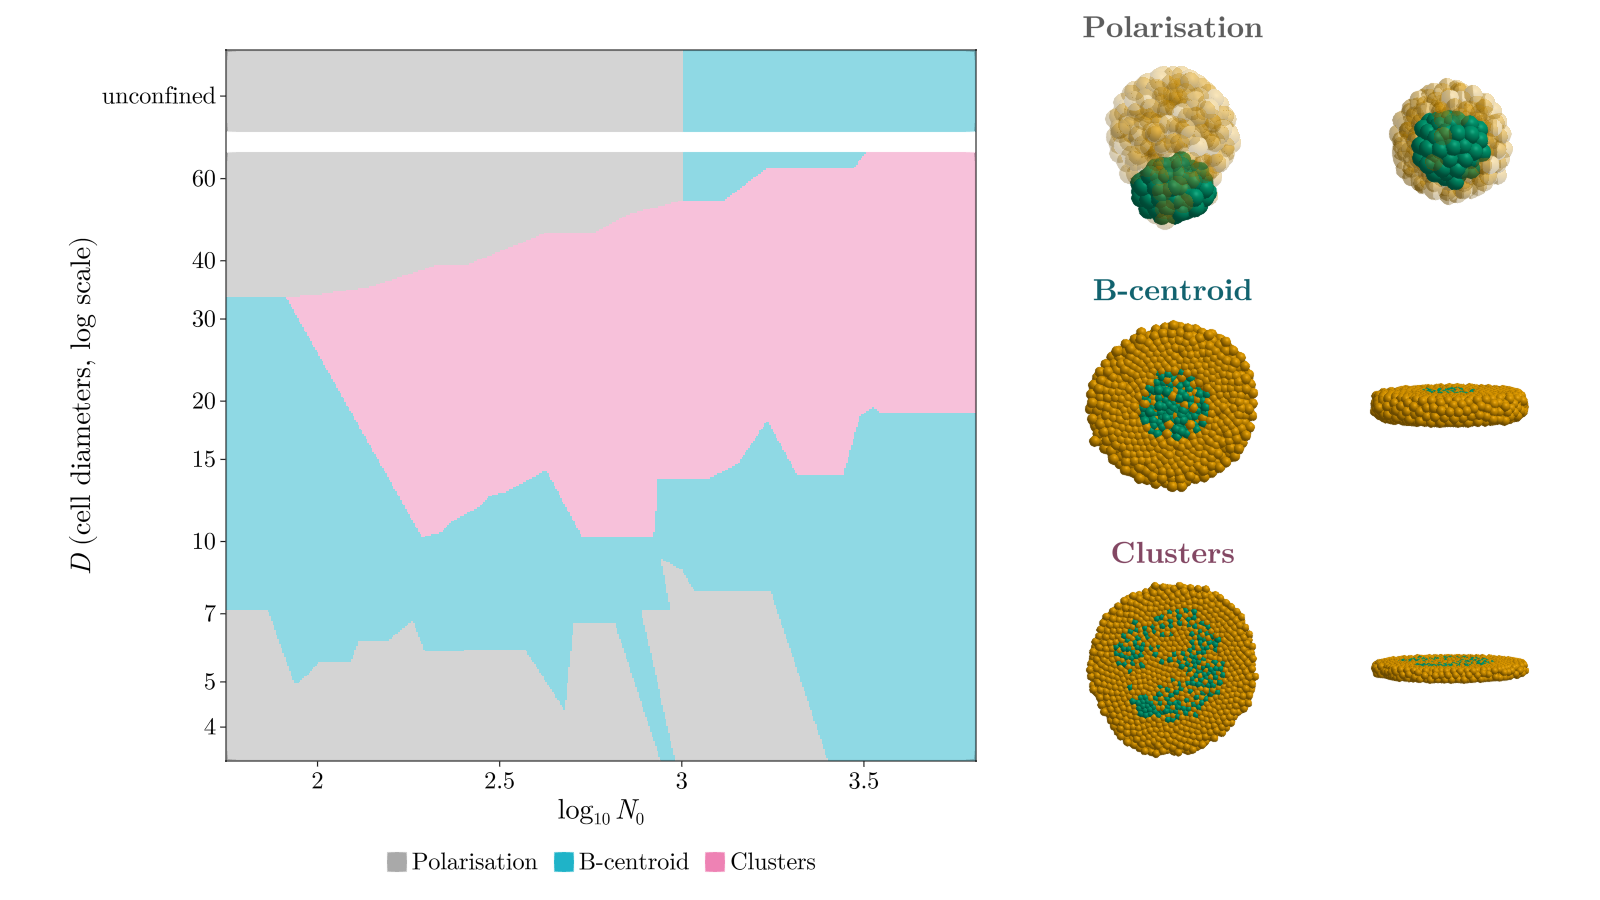
\includegraphics[width=\linewidth]{figures/phase_space_diameter.png}
    \caption{The same phase space against the diameter of the pancake at the moment of squeezing, in cell diameters (read when $20\%$ of the cells are $B$).}
    \label{phase-space-diameter}
\end{figure}

The outcome depends on when it is read. Figure~\ref{phase-space-late} shows the same simulations when only $12\%$ of the cells are $B$: the rings break into islands, larger aggregates polarise late, and the smallest monolayer patterns shrink back to a central cluster.

\begin{figure}[htbp]
    \centering
    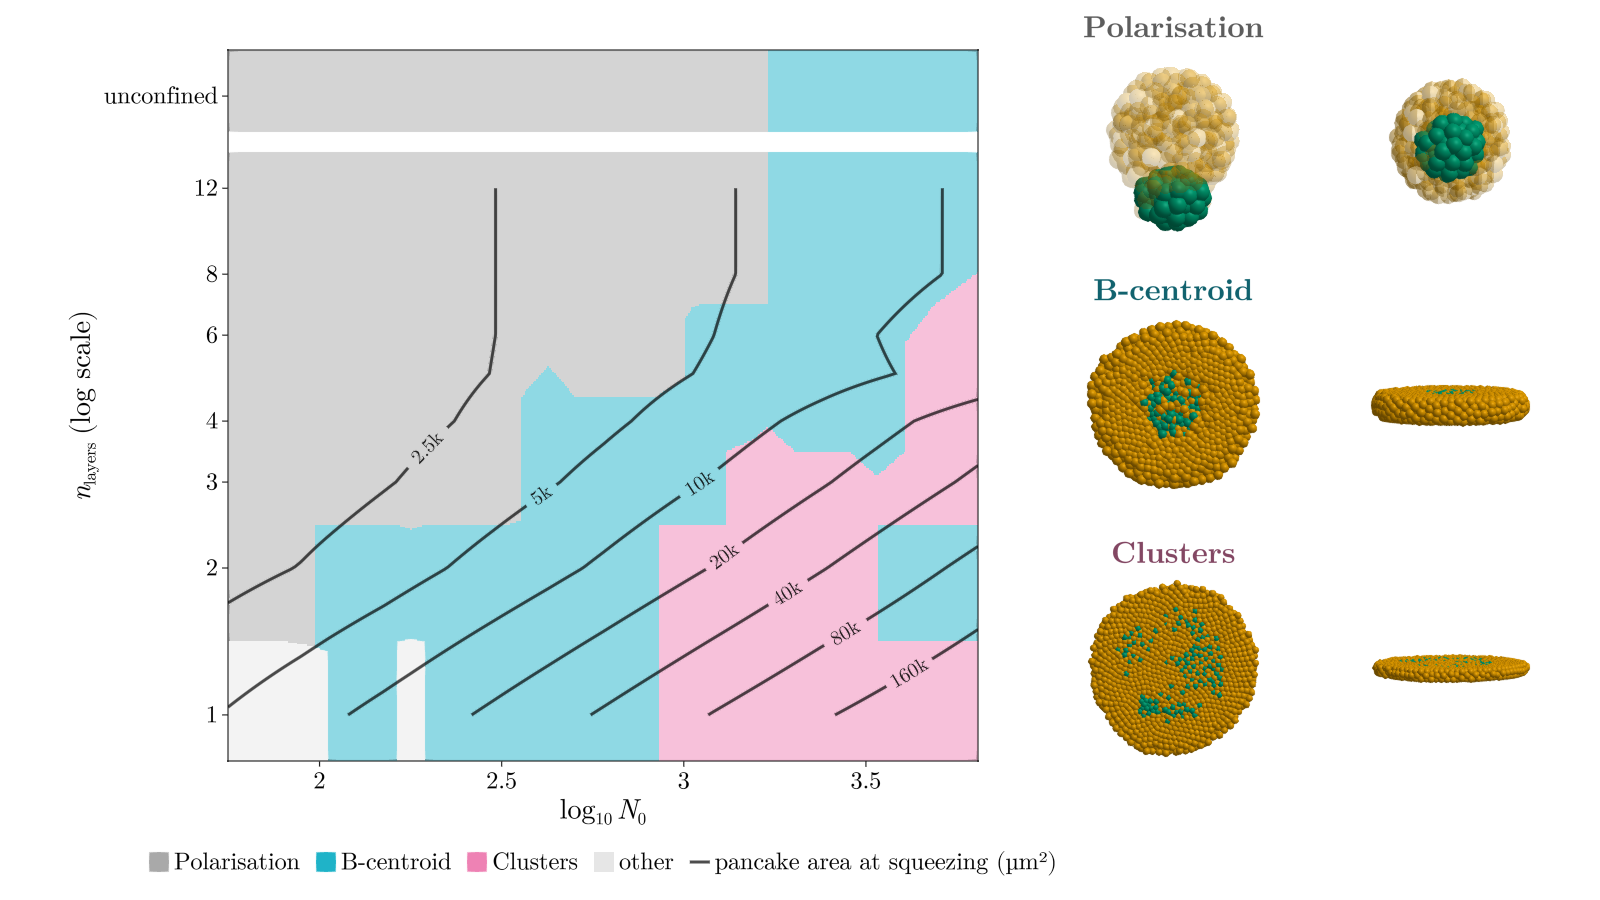
\includegraphics[width=\linewidth]{figures/phase_space_late.png}
    \caption{The same simulations, read when $12\%$ of the cells are $B$ (about $26$~h after the start of differentiation).}
    \label{phase-space-late}
\end{figure}

\subsection{Damköhler number}

The Damköhler number compares how fast cells differentiate with how fast they mix,
\begin{equation*}
    \mathrm{Da} = \frac{q\,\ell^2}{D},
\end{equation*}
where $q$ is the $B\to C$ rate, $D$ the diffusion coefficient of the cells and $\ell$ a length. If $\mathrm{Da}\gg1$, a cell differentiates long before it has moved a distance $\ell$, so the $B$ pattern is set where the cells already are. If $\mathrm{Da}\ll1$, cells mix over $\ell$ before they differentiate.

There is no noise in the model: cells move only because their neighbours divide and push them, and because differentiation changes the adhesion. We therefore measure $D$ in growing monolayers (one layer, $N_0 = 600$ and $2400$, two seeds each), saving one frame every time unit (4 minutes). Each cell is followed between two of its divisions, and only its in-plane displacement is used. The spreading of the slab as it grows is not diffusion, so it is removed from every displacement with an affine fit of the displacement field, $\mathbf u = A\,\mathbf r + \mathbf b$. As a check we also use the displacement relative to the neighbours within $5r$. Cells in the outer $20\%$ of the radius are left out. The mean squared displacement is then fitted with a straight line at long lag times (2 to 8~h),
\begin{equation*}
    \langle |\Delta \mathbf r|^2 \rangle = 4 D \tau + c .
\end{equation*}

The MSD is nearly linear from 4~min to 10~h (Figure~\ref{msd}). Between 2 and 8~h its log--log slope is $1.2$--$1.3$, so some directed motion remains: local flows that a single affine fit cannot remove, such as $B$ growing faster than $C$ and the sorting of the two. The sizes and the seeds agree within $20\%$:
\begin{equation*}
    D \approx 0.004\, r^2 \text{ per time unit} \approx 1.5~\mu\mathrm{m}^2/\mathrm{h}
\end{equation*}
for $B$ and $C$ cells alike ($0.0025$--$0.0034\, r^2$ per time unit relative to the neighbours).

With $q = 0.004667$ per time unit:
\begin{itemize}
    \item for $\ell$ one cell diameter, $\mathrm{Da} \approx 4$--$8$: a cell needs about $17$~h to move by its own diameter, longer than a $B$ cell lives ($1/q \approx 14$~h);
    \item for $\ell$ the radius of the pancake at squeezing, $\mathrm{Da} \approx 500$--$1000$ at $N_0=600$ and $2100$--$3800$ at $N_0=2400$.
\end{itemize}
Differentiation is therefore much faster than single-cell mixing at every size. For a fixed $D$, $\mathrm{Da}$ grows with the pancake area ($\mathrm{Da}\approx 0.015\,A/\mu\mathrm{m}^2$ for a monolayer), so the iso-area lines of the phase space are also lines of constant $\mathrm{Da}$, and the pattern threshold, at $A \approx 1.5\times10^4~\mu\mathrm{m}^2$, sits at $\mathrm{Da}\approx 200$.

\begin{remark}
    Over one frame (4~min) a cell moves about $0.04\,r \approx 0.2~\mu$m, i.e.\ $0.05~\mu$m/min. This is about 25 times slower than the instantaneous cell speed $V_0 \approx 1.25~\mu$m/min used to set the time unit $T_0 = R_0/V_0 = 4$~min.
\end{remark}

\begin{figure}[htbp]
    \centering
    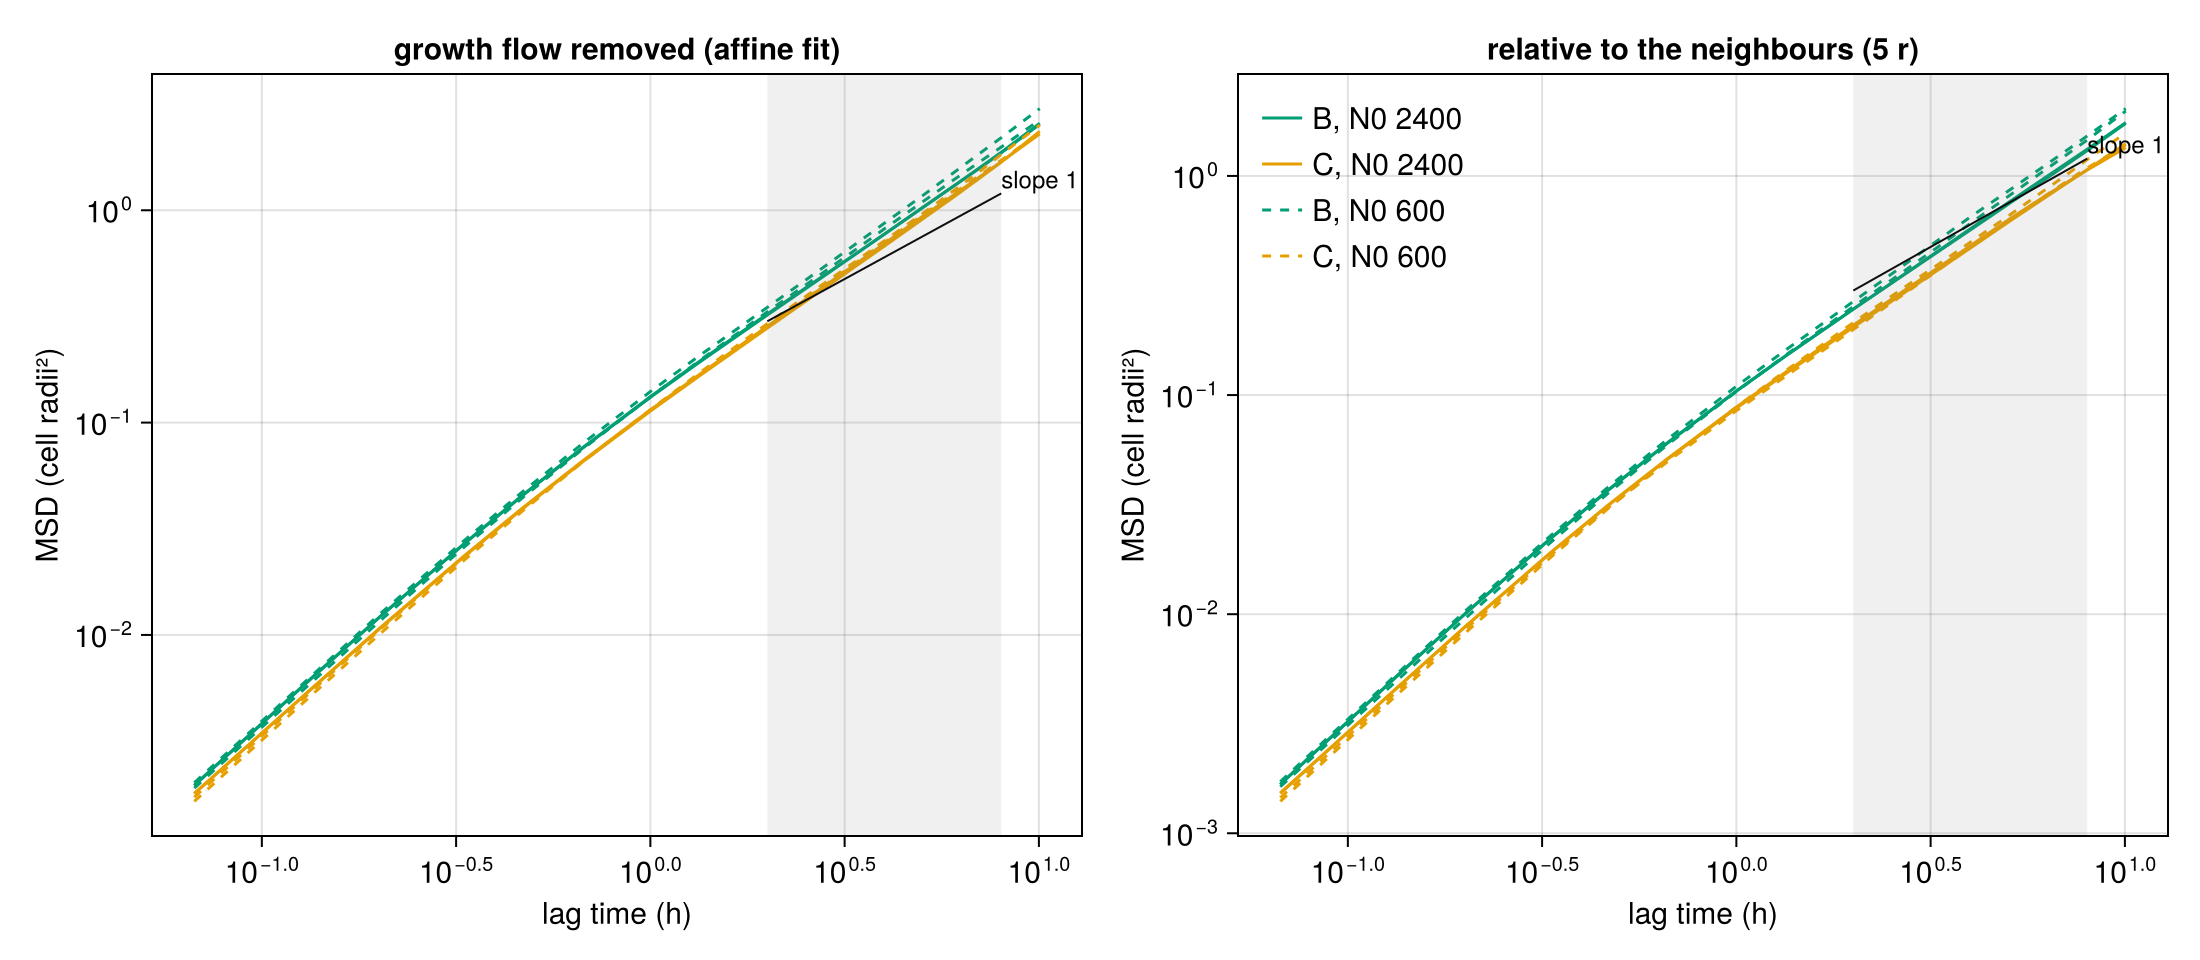
\includegraphics[width=\linewidth]{figures/msd.png}
    \caption{Mean squared displacement of $B$ (green) and $C$ (yellow) cells in growing monolayers ($N_0 = 600$ dashed, $2400$ solid). Left: growth flow removed with an affine fit; right: relative to the neighbours within $5r$. Shaded: the lag times of the fit.}
    \label{msd}
\end{figure}


\section{Open points and possible improvements}

\begin{enumerate}
    \item Large aggregates that are not confined (or confined with a wide gap) neither pattern nor polarise before $B$ runs out. A free $B$ core can always round up, so it does not break into islands.
    \item The transition from a central cluster to a ring is gradual: near the threshold the cluster becomes loose and starts opening. Where we put the cut moves the thresholds by about one step in $N_0$.
    \item The value $\mu_{BB}=1.9$ is close to the point where $B$ dissolves into $C$ ($\mu_{BB}=1.85$).
    \item More simulations per point would sharpen the boundaries; the phase space has 2 or 3 per point, and 1 at $N_0=4800$.
\end{enumerate}



\newpage
\section{Parameters}

Table~\ref{parameters} gives the parameters of the July report (old) and the ones used now (new). Values in \chg{red} have changed. Entries of the $A$ state are shown as $\unused$, since $A$ cells no longer exist; in the matrices the order is $A, B, C$.

{\small                                 % smaller font size for the table
\begin{xltabular}{\textwidth}{
    >{\centering\arraybackslash}p{0.08\textwidth}   % symbol
    X                                               % description
    >{\centering\arraybackslash}p{0.17\textwidth}   % Oriola et al. 2026
    >{\centering\arraybackslash}p{0.17\textwidth}   % old value
    >{\centering\arraybackslash}p{0.17\textwidth}   % new value
}
\caption{Parameters of Oriola et al.\ 2026 (DO, Tables S4--S5 and Supplementary Note S2), of the July report (old) and of this report (new). Values in \chg{red} have changed with respect to the July report.}
\label{parameters}\\
\hline
\textbf{Symbol} & {\textbf{Description}} & \textbf{DO} & \textbf{Sotiris} & \textbf{Current} \\      % header
\hline
\endfirsthead
\hline
\textbf{Symbol} & {\textbf{Description}} & \textbf{DO} & \textbf{Sotiris} & \textbf{Current} \\
\hline
\endhead
\hline
\endfoot
    $\Delta t$ & Timestep & 0.02 & 0.02 & \chg{0.015} \\
    $ r$ & Radius & 1 & 1 & 1 \\
     & Overlap factor & 0.3 & 0.3 & 0.3 \\
    $\alpha$ & Cell-ECM/cell-cell friction parameter & 0.9 & 0.9 & 0.9 \\
    $\tau_\text{div}^A$ & Average division time & 300 & 300 & \chg{-- (no $A$ cells)} \\
    $\tau_\text{div}^B$ & Average division time & 300 & 300 & 300 \\
    $\tau_\text{div}^C$ & Average division time & 750 & 750 & 750 \\
    $\sigma_\text{div}$ & Division time variability & 0.5 & 0.5 & 0.5 \\
    $N_\text{rel}$ & Division relaxation (neighbour counts) & 150 & -- & -- \\
    $\lambda$ & Global friction coefficient & 1 & 1 & 1 \\
    $\mu$ & Force range factor & 2 (all pairs) & $\begin{pmatrix}
        1.55 & 1.5 & 1.525 \\
        1.5  & 1.7 & 1.45 \\
        2.0  & 2.0 & 2.0
    \end{pmatrix}$ & $\begin{pmatrix}
        \unused & \unused & \unused \\
        \unused & \chg{1.9} & \chg{2} \\
        \unused & 2 & \chg{2.14}
    \end{pmatrix}$ \\
        & Neighbour range factor & -- &  1 & 1 \\
    $F_{rep}$ & Repulsion force & $\begin{pmatrix}
        3 & 3 & 3 \\
          & 3 & 3 \\
          &   & 5.1
    \end{pmatrix}$ & $\begin{pmatrix}
        3 & 3 & 3 \\
          & 3 & 3 \\
          &   & 5.1
    \end{pmatrix}$ & $\begin{pmatrix}
        \unused & \unused & \unused \\
          & \chg{4.5} & 3 \\
          &   & \chg{6}
    \end{pmatrix}$ \\
    $F_{att}$ & Attraction force & $\begin{pmatrix}
        6 & 6 & 2.4 \\
          & 6 & 1.6 \\
          &   & 4.8
    \end{pmatrix}$ & $\begin{pmatrix}
        6 & 6 & 2.4 \\
          & 6 & 1.6 \\
          &   & 4.8
    \end{pmatrix}$ & $\begin{pmatrix}
        \unused & \unused & \unused \\
          & \chg{6.4} & 1.6 \\
          &   & \chg{3}
    \end{pmatrix}$ \\
    $p$ & Fixed transition rate from $A$ to $B$ & 0.009333 & 0.009333 & \chg{-- (no $A$ cells)} \\
    $q$ & Fixed transition rate from $B$ to $C$ & 0.004667 & 0.004667 & 0.004667 \\
    $K$ & Feedback parameter & 0.2 & 0.2 & \chg{-- (no feedback)} \\
    $\lambda_\text{wall}$ & Plate friction (cells closer than 0.05 to a plate) & -- & -- & \chg{1.5} \\
     & Plates & -- & -- & \chg{rigid} \\
    $L$ & Plate gap & -- & -- & \chg{$2.1\,r \times$ layers} \\
    $\phi_B^0$ & Initial proportion of $B$ cells & -- & -- & \chg{0.6 (central core)} \\
     & Readout: proportion of $B$ cells & -- & -- & \chg{0.2} \\
    $n_i$ & Number of neighbours & & &  \\
    $n_i^X$ & Number of neighbours in state $X$ & & &  \\
    $\phi_X$ & Proportion of cells in state $X$ & & &  \\
    $T_0$ & Typical time scale & \SI{4}{\minute} & \SI{4}{\minute} & \SI{4}{\minute} \\
     & Time units per hour & 15 & -- & \chg{15} \\
    $R_0$ & Typical length scale & \SI{5}{\micro\meter} & \SI{5}{\micro\meter} & \SI{5}{\micro\meter} \\
    $F_0$ & Typical force scale & \SI{100}{\pico\newton} & \SI{20}{\pico\newton} & \SI{20}{\pico\newton} \\
\end{xltabular}
}

\textbf{Note on the old values.} They are the values in the table of the July report. The July simulations themselves used Sotiris' fusion set,
\begin{equation*}
    \mu = 2\begin{pmatrix} 1 & 0.91 & 1 \\ 0.91 & 1 & 1 \\ 1 & 1 & 1.07 \end{pmatrix}, \qquad
    F_\text{att} = 4\begin{pmatrix} 0.9 & 1 & 0.6 \\ 1 & 1.6 & 0.4 \\ 0.6 & 0.4 & 0.75 \end{pmatrix},
\end{equation*}
with $F_\text{rep}^{BB} = 3$ and $F_\text{rep}^{CC} = 5.1$, and Hookean plates. Compared with those, the only changes are $F_\text{rep}^{BB}$ ($3 \to 4.5$), $F_\text{rep}^{CC}$ ($5.1 \to 6$), $\mu_{BB}$ ($2 \to 1.9$), the plates (rigid, with friction $\lambda_\text{wall} = 1.5$) and the removal of the $A$ state. The $BC$ entries ($\mu_{BC}=2$, $F_\text{att}^{BC}=1.6$, $F_\text{rep}^{BC}=3$) and $q$ are unchanged. The typical time scale $T_0 = 2$~h does not match the $15$ time units per hour implied by $q$; it is worth checking.

\printbibliography

\end{document}
